% ============================================================
% Master rad — Evaluacija pouzdanosti velikih jezičkih modela
%              u automatskom ocenjivanju studentskih odgovora
% Autor: Svetozar Iković, Matematički fakultet, UB
%
% NAPOMENA: preambula je namerno minimalna i modularna — ako
% fakultet zahteva zvanični šablon, menja se samo ovaj fajl,
% a poglavlja u poglavlja/ ostaju netaknuta.
% ============================================================
\documentclass[12pt,a4paper]{article}

% --- Jezik i pismo (srpski, latinica) ---
% Preambula radi i pod pdfLaTeX-om (inputenc/fontenc) i pod
% XeTeX/LuaTeX-om (fontspec) — Tectonic koristi XeTeX.
\usepackage{iftex}
\ifPDFTeX
  \usepackage[utf8]{inputenc}
  \usepackage[T1]{fontenc}
  \usepackage{lmodern}
\else
  \usepackage{fontspec} % podrazumevani font je Latin Modern
\fi
\usepackage[serbian]{babel}

% --- Matematika, grafika, tabele ---
\usepackage{amsmath}
\usepackage{graphicx}
\usepackage{booktabs}
\usepackage{makecell}
\usepackage{multirow}

% --- Prompt kutije (kao u ComSIS radu) ---
\usepackage[most]{tcolorbox}
\usepackage{enumitem}
\tcbset{
  promptbox/.style={
    colback=gray!3,
    colframe=black,
    boxrule=0.4pt,
    arc=2pt,
    left=6pt, right=6pt, top=6pt, bottom=6pt,
    breakable
  }
}

% --- Dijagram arhitekture ---
\usepackage{tikz}
\usetikzlibrary{arrows.meta, positioning, shapes.geometric}

% --- Kod ---
\usepackage{listings}
\usepackage{xcolor}
\lstset{
  basicstyle=\ttfamily\small,
  breaklines=true,
  frame=single,
  framerule=0.3pt,
  captionpos=b,
  showstringspaces=false
}

% --- Ostalo ---
\usepackage{url}
\usepackage[hidelinks]{hyperref}

% Marker za nedovršene delove — pretragom po \todo lako se
% nalazi šta je preostalo; pre predaje ne sme ostati nijedan.
\newcommand{\todo}[1]{\textcolor{red}{\textbf{[TODO: #1]}}}

% Razmak i uvlačenje pasusa
\usepackage{setspace}
\onehalfspacing

\begin{document}

% ------------------------------------------------------------
% Naslovna strana
% ------------------------------------------------------------
\begin{titlepage}
    \centering
    \vspace*{2cm}
    {\Large\bfseries Univerzitet u Beogradu\\Matematički fakultet\par}
    \vspace{3cm}
    {\LARGE\bfseries Evaluacija pouzdanosti velikih jezičkih modela u automatskom ocenjivanju studentskih odgovora\par}
    \vspace{1cm}
    {\large Master rad\par}
    \vspace{2cm}
    {\Large Autor: Svetozar Iković\par}
    \vfill
    {\large Mentor: dr Jelena Graovac\par}
    \vspace{1cm}
    {\large Beograd, 2026.\par}
\end{titlepage}

% ------------------------------------------------------------
% Zahvalnica, rezime, sadržaj
% ------------------------------------------------------------
\section*{Zahvalnica}
Zahvaljujem se...

\newpage

\section*{Rezime}

Ubrzani razvoj veštačke inteligencije i velikih jezičkih modela (LLM) menja praksu provere znanja u visokom obrazovanju, naročito u ocenjivanju pitanja otvorenog tipa.
Tradicionalno ocenjivanje je vremenski zahtevno, sklono nedoslednosti i teško skalabilno za velike grupe studenata.
Veliki jezički modeli, zahvaljujući sposobnosti razumevanja i rezonovanja o prirodnom jeziku, pružaju priliku za unapređenje efikasnosti, doslednosti i učestalosti povratnih informacija.
U ovom radu predstavljen je EduGrader, višemodelska platforma otvorenog koda za ocenjivanje koja objedinjuje više velikih jezičkih modela: GPT-4o, GPT-4o-mini, DeepSeek-Chat, GPT-5.1 i DeepSeek-Reasoner.
EduGrader podržava tri nivoa strogosti ocenjivanja (blag, neutralan, strog) i generiše numeričke ocene sa sažetim obrazloženjima koja ističu ispravno rezonovanje, koncepte koji nedostaju i greške.
Sistem radi u dva režima: režimu sa zadatim referentnim odgovorom (PRA), vođenom rešenjima nastavnika, i režimu sa generisanim referentnim odgovorom (GRA), koji referentne odgovore automatski konstruiše iz nastavnih materijala.
Svi eksperimenti sprovedeni su na srpskom --- jeziku sa ograničenim resursima, slabo zastupljenom u podacima za obučavanje savremenih modela --- čime se istraživanje ocenjivanja uz podršku veštačke inteligencije proširuje izvan dominantnog engleskog konteksta.
EduGrader je evaluiran na 686 autentičnih studentskih odgovora sa šest univerzitetskih kurseva na dve institucije, uključujući tekstualna objašnjenja i odgovore u obliku koda.
U najboljoj konfiguraciji sistem postiže Pirsonov koeficijent korelacije od 0{,}90 sa ljudskim ocenjivačima, uz smanjenje opterećenja nastavnika i poboljšanje pouzdanosti, pri čemu je namenjen kao pomoć nastavnicima, a ne kao njihova zamena.

\medskip
\noindent\textbf{Ključne reči:} automatsko ocenjivanje, obrazovanje, veliki jezički modeli, veštačka inteligencija.
\newpage


\tableofcontents
\newpage

% ------------------------------------------------------------
% Poglavlja
% ------------------------------------------------------------
% 1. Uvod
\section{Uvod}
\label{sec:uvod}

Ocenjivanje retko predstavlja najzanimljiviji deo nastave, ali često neprimetno oblikuje način na koji studenti uče.
Kada je povratna informacija pravovremena i konkretna, studenti mogu da prepoznaju i isprave nesporazume pre nego što se oni ustale.
Kada kasni, kada je neodređena ili nedosledna, provera znanja postaje formalnost, a učenje usporava.
Ovaj izazov je posebno vidljiv na velikim univerzitetskim kursevima, gde nastavnici i saradnici moraju da ocene stotine odgovora otvorenog tipa u kratkim rokovima.
Za razliku od pitanja sa ponuđenim odgovorima, kratka objašnjenja i mini-eseji ne mogu se proveriti prostim uparivanjem obrazaca.
Oni zahtevaju tumačenje: prepoznavanje delimično ispravnog rezonovanja, razlikovanje sitnih jezičkih nepreciznosti od konceptualnih praznina i odlučivanje koliko neki propust treba da utiče na ocenu.
Zbog toga ocenjivanje odgovora otvorenog tipa ostaje skupo i teško skalabilno.
Ono je, takođe, sklono nedoslednosti: čak i uz detaljna uputstva za ocenjivanje, dva ocenjivača mogu isti odgovor protumačiti različito, naročito kada su odgovori dvosmisleni, pisani u žurbi ili strukturno nejasni~\cite{jonsson2007use,stemler2004comparison,brookhart2016century}.
Za nastavnike ovo opterećenje ograničava koliko često mogu da koriste bogatija pitanja zasnovana na objašnjenjima.
Za studente to često znači da povratna informacija stiže prekasno da bi bila korisna --- ili ne stiže uopšte.

Ranije generacije sistema za automatsku proveru znanja dobro su funkcionisale samo kada su odgovori bili strogo ograničeni, kao kod testova sa ponuđenim odgovorima, pitanja dopunjavanja ili kratkih odgovora sa predvidljivom formulacijom~\cite{shermis2003automated,brew2013automated,ramesh2022automated}.
Napredak u obradi prirodnog jezika proširio je ove mogućnosti, ali su se mnogi pristupi i dalje oslanjali na obimno ručno projektovanje atributa, uske domene ili velike označene skupove podataka~\cite{sebastiani2002machine,collobert2008unified,banko2001scaling}.
Savremeni veliki jezički modeli (engl. \emph{large language models}, LLM), međutim, označavaju prekretnicu: oni mogu neposredno da tumače slobodan tekst i rezonuju o njegovom značenju.
Time je postalo izvodljivo projektovati alate koji ocenjuju odgovore otvorenog tipa, obrazlažu dodeljene ocene prirodnim jezikom i ukazuju na ono što u odgovoru nedostaje, a ne samo na ono što je pogrešno~\cite{kasneci2023chatgpt,zhai2023chatgpt}.

\subsection{Motivacija}

Primarni cilj ovog rada jeste unapređenje obrazovnog procesa kroz pouzdanu automatizaciju ocenjivanja.
Postojeći način provere znanja zahteva značajnu angažovanost nastavnika, što dovodi do kašnjenja povratnih informacija i ograničava učestalost testiranja.
Pouzdan automatizovani sistem za ocenjivanje omogućio bi:
\begin{itemize}
    \item \textbf{Povećanje učestalosti testiranja:} redovnije provere znanja omogućavaju studentima da kontinuirano prate svoj napredak i identifikuju oblasti koje zahtevaju dodatni rad.
    \item \textbf{Unapređenje procesa učenja:} automatsko ocenjivanje pruža brzu i detaljnu analizu odgovora, čime studenti dobijaju uvid u sopstvene greške dok je gradivo još sveže.
    \item \textbf{Smanjenje opterećenja nastavnika:} automatizacijom rutinskog dela ocenjivanja oslobađa se vreme koje nastavnici mogu usmeriti ka individualnoj podršci studentima.
\end{itemize}

Ipak, upotreba velikih jezičkih modela u ocenjivanju otvara važna praktična i pedagoška pitanja.
Koliko su njihove ocene dosledne kroz različite predmete i tipove pitanja?
Mogu li nastavnici kalibrisati strogost ocenjivanja prema očekivanjima konkretnog kursa?
Šta se dešava kada potpun referentni odgovor nije dostupan?
I, što je ključno, kako očuvati ljudsku odgovornost za konačne ocene, a iskoristiti efikasnost automatizacije?

\subsection{Sistem EduGrader i doprinosi rada}

U ovom radu predstavljen je EduGrader, platforma za ocenjivanje uz podršku veštačke inteligencije, projektovana za proveru znanja putem pitanja otvorenog tipa u visokom obrazovanju, pod nadzorom nastavnika.
EduGrader objedinjuje više velikih jezičkih modela --- GPT-4o\footnote{\url{https://platform.openai.com/docs/models/gpt-4o}}, GPT-4o-mini\footnote{\url{https://platform.openai.com/docs/models/gpt-4o-mini}}, DeepSeek-Chat\footnote{\url{https://api-docs.deepseek.com/}} i dva modela usmerena na rezonovanje, GPT-5.1\footnote{\url{https://platform.openai.com/docs/models/gpt-5}} i DeepSeek-Reasoner\footnote{\url{https://api-docs.deepseek.com/guides/reasoning\_model}} --- u jedinstven, transparentan tok ocenjivanja koji prioritet daje kontroli nastavnika.
Sistem podržava tri profila strogosti ocenjivanja --- blag, neutralan i strog --- što odražava stvarnu nastavnu praksu, u kojoj neki kursevi nagrađuju delimično ispravno rezonovanje, dok drugi zahtevaju preciznu terminologiju i potpuna rešenja.

EduGrader nudi dva komplementarna režima ocenjivanja:
\begin{itemize}
    \item \textbf{Režim sa zadatim referentnim odgovorom} (engl. \emph{provided-reference-answer}, PRA), u kome se studentski odgovori porede sa referentnim odgovorima koje je pripremio nastavnik (po potrebi dopunjenim napomenama za ocenjivanje).
    \item \textbf{Režim sa generisanim referentnim odgovorom} (engl. \emph{generated-reference-answer}, GRA), u kome sistem najpre sam konstruiše referentni odgovor na osnovu nastavnih materijala --- beležaka sa predavanja, skripti i udžbenika --- a zatim studentske odgovore ocenjuje u odnosu na tako generisani standard.
\end{itemize}

U oba režima izlaz sistema ne čini samo numerička ocena (0--10), već i jasno obrazloženje koje ukazuje na jake strane odgovora, koncepte koji nedostaju i praznine u rezonovanju.
Cilj je povratna informacija koja je studentima upotrebljiva, a nastavnicima proverljiva, umesto ocene koja dolazi iz „crne kutije''.

Svi eksperimenti sprovedeni su na srpskom jeziku --- jeziku sa ograničenim resursima, slabo zastupljenom u podacima na kojima se veliki jezički modeli obučavaju --- čime se istraživanje ocenjivanja uz podršku veštačke inteligencije proširuje izvan dominantnog engleskog konteksta.
Sistem je evaluiran na 686 autentičnih studentskih odgovora prikupljenih na dva univerziteta i šest kurseva, koji obuhvataju različite tipove odgovora: kratke činjeničke odgovore, otvorena tekstualna objašnjenja i odgovore u obliku koda.
Rezultati pokazuju da PRA režim daje stabilnije ishode od GRA režima i da se modeli usmereni na rezonovanje najbolje slažu sa ljudskim ocenjivačima.
U najboljoj konfiguraciji (GPT-5.1, neutralna strogost) EduGrader postiže Pirsonov koeficijent korelacije (PCC) od 0{,}90 u odnosu na ljudsko ocenjivanje.

Konačno, EduGrader je zamišljen kao asistent za ocenjivanje, a ne kao zamena za sud nastavnika.
On smanjuje repetitivno opterećenje i povećava doslednost, ali ljudski nadzor ostaje neophodan za dvosmislena pitanja, očekivanja specifična za disciplinu i granične slučajeve.
Iz tog razloga EduGrader sledi princip čoveka u petlji (engl. \emph{human-in-the-loop}) i objavljen je kao softver otvorenog koda, čime se podstiču transparentnost, reproducibilnost i prilagodljivost različitim institucijama.

\subsection{Struktura rada}

Ostatak rada organizovan je na sledeći način.
U poglavlju~\ref{sec:pregled} dat je pregled oblasti i srodnih istraživanja primene veštačke inteligencije u ocenjivanju.
Poglavlje~\ref{sec:aplikacija} opisuje veb aplikaciju EduGrader i sloj za integraciju jezičkih modela, a poglavlje~\ref{sec:pipeline} sistem za automatizovanu evaluaciju modela kojim su sprovedeni eksperimenti.
U poglavlju~\ref{sec:metodologija} predstavljena je metodologija evaluacije --- korišćene metrike, skupovi podataka i konfiguracije modela.
Poglavlje~\ref{sec:rezultati} donosi rezultate eksperimenata, uključujući poređenje PRA i GRA režima, analizu uticaja temperature, Bland--Altmanovu analizu slaganja i analizu stabilnosti ocenjivanja kroz višestruka pokretanja.
U poglavlju~\ref{sec:diskusija} rezultati su upoređeni sa prethodnim istraživanjima i razmotreni su pravci budućeg rada, dok poglavlje~\ref{sec:zakljucak} zaključuje rad.
Dodatak~\ref{app:promptovi} sadrži šablone promptova korišćene u eksperimentima i reprezentativne primere ocenjivanja.

% 2. Pregled oblasti i srodni radovi
\section{Pregled oblasti i srodni radovi}
\label{sec:pregled}

Istraživanja primene veštačke inteligencije u obrazovanju otkrivaju jasnu evoluciju od rane automatizacije zasnovane na pravilima ka adaptivnim sistemima sposobnim da tumače i generišu složene odgovore nalik ljudskim.
Osnovne definicije opisuju veštačku inteligenciju kao računarske sisteme projektovane da obavljaju kognitivne funkcije poput učenja, rezonovanja i rešavanja problema~\cite{baker2019educ}.
U obrazovnom kontekstu, veštačka inteligencija obuhvata širok skup tehnologija koje zajedno omogućavaju personalizovanija i adaptivnija okruženja za učenje~\cite{zawacki2019systematic}.
Brojne studije i sistematski pregledi naglašavaju njen potencijal da unapredi ishode učenja, proširi dostupnost obrazovanja i podrži efikasnije korišćenje nastavnih resursa~\cite{yuskovych2022application,zhang2023study}.
Noviji napredak velikih jezičkih modela dodatno je proširio ove mogućnosti.
Za razliku od ranijih pristupa zasnovanih na obradi prirodnog jezika, koji su se oslanjali na ručno projektovane atribute ili obučavanje za konkretan domen, veliki jezički modeli mogu neposredno da obrađuju slobodan tekst i rezonuju o značenju na višem nivou apstrakcije.
Zbog toga se sve više ispituju za nastavu usmerenu na učenika, automatsko generisanje sadržaja i nove oblike provere znanja u širokom spektru obrazovnih domena~\cite{zhang2023study}.

Empirijske studije koje ispituju ocenjivanje uz podršku velikih jezičkih modela daju mešovite, ali informativne rezultate.
Kuli i Jusuf~\cite{kooli2025transforming} sproveli su empirijsko istraživanje ocenjivanja uz pomoć ChatGPT-a na skupu od 25 studentskih radova iz kohorte od približno 100 studenata druge godine na kursu iz društvenih nauka.
U njihovoj eksperimentalnoj postavci, i ljudski ocenjivači i ChatGPT nezavisno su evaluirali radove, što je omogućilo neposredno poređenje automatskog i ljudskog ocenjivanja.
Studija je prijavila umerenu korelaciju između ocena veštačke inteligencije i ljudskih ocena (koeficijent korelacije približno 0{,}45), što sugeriše da model može da aproksimira opšte obrasce ocenjivanja, ali da značajne razlike ostaju u pojedinačnim evaluacijama.
Autori dalje ističu da ChatGPT može pružiti korisnu povratnu informaciju i ubrzati proces ocenjivanja, ali da njegova automatska priroda može ograničiti kontekstualno razumevanje nijansiranih studentskih argumenata.
Takođe naglašavaju potencijalne rizike, poput produbljivanja obrazovnih nejednakosti, i potrebu za institucionalnim okvirima koji obezbeđuju transparentnost, nadzor i ublažavanje pristrasnosti pri uvođenju alata za ocenjivanje zasnovanih na veštačkoj inteligenciji.

Slično tome, Lundgren~\cite{lundgren2024large} je ispitao performanse modela GPT-4 u ocenjivanju eseja u visokom obrazovanju, na skupu od 60 eseja master nivoa iz političkih nauka koje su prethodno ocenili univerzitetski nastavnici.
Studija je uporedila ocene koje je predložio GPT-4 sa ocenama ljudskih ocenjivača i utvrdila da su prosečne ocene modela u velikoj meri usklađene sa evaluacijama nastavnika.
Analiza je, međutim, otkrila nižu pouzdanost među ocenjivačima (između modela i ljudi), što ukazuje da model može aproksimirati agregirane trendove ocenjivanja, ali se muči da dosledno replicira fino ljudsko rasuđivanje.
Pored toga, model je pokazao obrazac ocenjivanja sklon izbegavanju rizika i tendenciju da se oslanja na opšte karakteristike eseja, poput kvaliteta jezika, umesto da se u potpunosti prilagodi detaljnim rubrikama za ocenjivanje.
Eksperimenti sa izmenjenim promptovima i uputstvima za ocenjivanje doneli su samo ograničena poboljšanja, što sugeriše da su tadašnji sistemi za ocenjivanje zasnovani na velikim jezičkim modelima relativno neosetljivi na suptilne varijacije u kriterijumima evaluacije.

Za razliku od ocenjivanja eseja, Jukjevič~\cite{jukiewicz2024future} je istražio primenu ChatGPT-a za ocenjivanje programerskih zadataka na petnaestonedeljnom kursu programiranja u Python-u sa 67 studenata osnovnih studija kognitivnih nauka.
Kroz devet programerskih zadataka, i nastavnik i ChatGPT nezavisno su evaluirali studentske radove, što je omogućilo poređenje doslednosti ocenjivanja i kvaliteta povratnih informacija.
Rezultati su pokazali snažnu pozitivnu korelaciju između ocena ChatGPT-a i evaluacija nastavnika, mada je sistem težio da dodeljuje nešto strože ocene.
Studija je takođe prijavila odličnu ponovljivost rezultata ocenjivanja kroz višestruka pokretanja, sa zanemarljivim varijacijama između iteracija.
Pored numeričkih ocena, ChatGPT je bio u stanju da proceni ispravnost koda, proveri poštovanje standarda kodiranja poput smernica PEP8 i generiše detaljnu povratnu informaciju u roku od nekoliko sekundi, značajno smanjujući vreme potrebno za ručno ocenjivanje.
Uprkos tome, autor identifikuje i nekoliko ograničenja, uključujući mogućnost halucinirananih grešaka, troškove korišćenja API-ja i povremene nedoslednosti u ocenjivanju koje zahtevaju proveru nastavnika.
Studija zaključuje da ChatGPT može poslužiti kao vredan komplementaran alat za automatsku procenu koda i generisanje povratnih informacija, ali da ljudski nadzor ostaje neophodan za obezbeđivanje pouzdanosti i pravednosti.

Ovi nalazi podržavaju šire dokaze koji ukazuju da pouzdanost ocenjivanja velikim jezičkim modelima zavisi od tipa zadatka: slaganje sa ljudskim ocenjivačima teži da bude više u domenima sa strukturiranim odgovorima, poput definicija, formula ili fragmenata koda, dok performanse opadaju kod subjektivnih ili otvorenih pisanih zadataka~\cite{tomic2022ai,vittorini2021ai}.
Na primer, u radu~\cite{pinto2023large} evaluiran je GPT-3 na odgovorima otvorenog tipa profesionalaca iz industrije i uočene su snažne korelacije sa ekspertskim ocenama, pod uslovom da su kriterijumi jasno definisani i kontekstualno utemeljeni.
Izvan numeričkog ocenjivanja, više studija ističe širu ulogu veštačke inteligencije u podršci procesima provere znanja.
Pokazano je da sistemi zasnovani na veštačkoj inteligenciji mogu da generišu adaptivne aktivnosti učenja, isporučuju personalizovanu povratnu informaciju i podrže i formativno i sumativno ocenjivanje zasnovano na individualnim karakteristikama učenika~\cite{diwan2023ai,luckin2016intelligence}.
Inteligentni tutorski sistemi i srodni pristupi nastoje da aproksimiraju individualnu nastavnu podršku uz istovremeno povećanje doslednosti i skalabilnosti evaluacije~\cite{conati2009intelligent,garcia2018social}.
Istovremeno, kritičke perspektive upozoravaju na „zamagljivanje'' odgovornosti u automatskom ocenjivanju, gde procesi donošenja odluka postaju neprozirni, a odgovornost razvodnjena~\cite{swiecki2022assessment}.
Zbog toga transparentnost, objašnjivost, privatnost podataka i kvalitet povratnih informacija ostaju centralne teme konceptualnih analiza ocenjivanja podržanog veštačkom inteligencijom~\cite{kumar2023faculty}.

Kroz ovu literaturu provlači se dosledan zaključak: velike jezičke modele najbolje je razumeti kao pomoćne alate koji automatizuju rutinske aspekte ocenjivanja i povratnih informacija, dok ljudski nastavnici ostaju nezamenljivi za pedagoško rasuđivanje, kontekstualno tumačenje i rešavanje dvosmislenih ili graničnih slučajeva~\cite{van2022applications,zawacki2019systematic}.
Shodno tome, pristupi koji kombinuju automatizaciju sa nadzorom čoveka u petlji, podesivim ponašanjem ocenjivanja i interpretabilnom povratnom informacijom najbliže odgovaraju aktuelnim preporukama u literaturi.
Upravo ova razmatranja motivišu dizajn sistema koji prioritet daju kontroli nastavnika, transparentnosti i prilagodljivosti --- principima koji neposredno oblikuju dizajn platforme EduGrader predstavljene u ovom radu.

% 3. Veb aplikacija EduGrader
\section{Veb aplikacija EduGrader}
\label{sec:aplikacija}

EduGrader je veb aplikacija za automatsko ocenjivanje odgovora otvorenog tipa sa studentskih ispita pomoću velikih jezičkih modela.
Predstavlja produkcioni deo sistema, namenjen svakodnevnoj upotrebi u nastavi, i implementirana je kao modularna platforma organizovana u tri sloja (slika~\ref{fig:architecture}):

\begin{itemize}
    \item \textbf{Klijentski sloj.} Jednostranična aplikacija (SPA) izgrađena u tehnologijama React~19 i TypeScript, koju poslužuje Nginx server.
    Pruža interaktivne prikaze za nastavnike i studente, uključujući otpremanje CSV datoteka, izbor modela i parametara i prikaz rezultata.
    Kroz ovaj interfejs nastavnici otpremaju studentske odgovore, biraju željeni jezički model, režim ocenjivanja (PRA ili GRA) i nivo strogosti, nakon čega sistem generiše predloge ocena sa obrazloženjima za svaki odgovor.
    Autentifikacija se obavlja putem JWT tokena (engl. \emph{JSON Web Token}) sa kontrolom pristupa zasnovanom na ulogama.
    \item \textbf{Serverski sloj.} REST API izgrađen u tehnologijama Python~3, Django~5.1 i Django REST Framework.
    Odgovoran je za generisanje promptova, izvršavanje modela, parsiranje izlaza i upravljanje konfiguracijom ocenjivanja.
    \item \textbf{Sloj baze podataka.} Realizovan kroz Django ORM, sa entitetima za kurseve, testove, pitanja, studentske odgovore i ocene.
    Čuva ocene, povratne informacije, promptove i metapodatke, čime podržava reproducibilnost i različite vrste analiza.
\end{itemize}

Ovakav slojeviti dizajn omogućava da se logika ocenjivanja i ponašanje modela razvijaju nezavisno od korisničkog interfejsa, uz očuvanje sledivosti svih odluka o ocenjivanju.
Klijentski i serverski deo komuniciraju isključivo preko REST API-ja.

% --- DIJAGRAM ARHITEKTURE (TikZ) ---
\begin{figure}[htbp]
\centering
\resizebox{\textwidth}{!}{%
\begin{tikzpicture}[
    node distance=0.6cm and 0.8cm,
    box/.style={draw, rounded corners=3pt, minimum height=0.9cm, text centered, font=\small},
    arr/.style={-{Stealth[length=2.5mm]}, thick},
    darr/.style={-{Stealth[length=2.5mm]}, thick, densely dashed},
    lbl/.style={font=\scriptsize, midway, fill=white, inner sep=1pt},
]

% ---- Klijentski sloj ----
\node[box, fill=red!8, minimum width=3.8cm, minimum height=1.6cm] (fe) {};
\node[font=\small\bfseries, anchor=north] at (fe.north) {Klijentski sloj};
\node[font=\scriptsize, anchor=south] at (fe.south) {React 19 + TypeScript};
\node[font=\scriptsize] at (fe.center) {UI za ocenjivanje \textbar{} JWT};

% ---- Serverski sloj ----
\node[box, fill=red!8, minimum width=5.6cm, minimum height=3.4cm, right=2.2cm of fe] (be) {};
\node[font=\small\bfseries, anchor=north] at (be.north) {Serverski sloj};
\node[font=\scriptsize, anchor=north, yshift=-3mm] at (be.north) {Django 5.1 + DRF (Python 3)};

% Unutrašnje komponente
\node[box, fill=red!15, minimum width=4.4cm, font=\scriptsize] at ([yshift=-2mm]be.center) (gm) {Modul za ocenjivanje};
\node[box, fill=red!22, minimum width=4.4cm, font=\scriptsize, below=0.3cm of gm] (factory) {Fabrika LLM integracija};

% ---- Baza podataka ----
\node[box, fill=yellow!15, minimum width=2.8cm, minimum height=1.2cm, below=1.4cm of be] (db) {};
\node[font=\small\bfseries] at ([yshift=1.5mm]db.center) {Baza podataka};
\node[font=\scriptsize] at ([yshift=-3mm]db.center) {kursevi, testovi, ocene};

% ---- LLM API-ji ----
\node[box, fill=red!8, minimum width=3.4cm, minimum height=1.1cm, align=center, right=2.2cm of factory, yshift=0.8cm]
  (openai) {\scriptsize OpenAI API\\[-1pt]\tiny gpt-4o-mini, gpt-4o, gpt-5.1};

\node[box, fill=red!8, minimum width=3.4cm, minimum height=1.1cm, align=center, right=2.2cm of factory, yshift=-0.8cm]
  (deepseek) {\scriptsize DeepSeek API\\[-1pt]\tiny deepseek-chat, deepseek-reasoner};

% ---- DVC pipeline ----
\node[box, fill=purple!8, minimum width=3.8cm, minimum height=1.6cm, below=1.4cm of fe] (pipe) {};
\node[font=\small\bfseries, anchor=north] at (pipe.north) {DVC \emph{pipeline}};
\node[font=\scriptsize] at (pipe.center) {Grupni eksperimenti};
\node[font=\scriptsize, anchor=south] at (pipe.south) {spajanje \textrightarrow{} ocenjivanje};

% ---- Strelice ----
\draw[arr] (fe.east) -- node[lbl, above] {REST API} (be.west |- fe.east);
\draw[arr] (be.south) -- node[lbl, right] {ORM} (db.north);
\draw[arr] (factory.east) -- ++(0.6,0) |- (openai.west);
\draw[arr] (factory.east) -- ++(0.6,0) |- (deepseek.west);
\draw[darr] (pipe.east) -- ++(0.8,0) |- node[lbl, below, pos=0.25] {koristi} (factory.west);

\end{tikzpicture}%
}
\caption{Arhitektura sistema EduGrader.
Klijentski sloj komunicira sa serverskim slojem preko REST API-ja.
Serverski sloj pristupa jezičkim modelima kroz jedinstven integracioni sloj (projektni obrazac fabrika) koji apstrahuje API-je pojedinačnih provajdera.
Sistem za automatizovanu evaluaciju (poglavlje~\ref{sec:pipeline}) koristi isti integracioni sloj za grupne eksperimente.}
\label{fig:architecture}
\end{figure}

\subsection{Klijentska aplikacija}
\label{sec:webapp}

Klijentska aplikacija realizovana je kao jednostranična aplikacija u biblioteci React (verzija 19) sa TypeScript jezikom, uz Vite kao alat za izgradnju i razvojno okruženje.
Rutiranje je rešeno bibliotekom React Router, kroz koju je aplikacija podeljena na dva modula sa odvojenim pravima pristupa:

\begin{itemize}
    \item \textbf{Nastavnički modul} omogućava pregled predmeta, kreiranje testova i pitanja, pokretanje automatskog ocenjivanja i pregled ocenjenih studentskih testova sa predlozima ocena i obrazloženjima modela.
    \item \textbf{Studentski modul} omogućava pregled nadolazećih testova, izradu testa i uvid u rezultate već urađenih testova.
\end{itemize}

Autentifikacija koristi JWT tokene koji se čuvaju u \emph{session storage}-u pregledača; uloge (nastavnik ili student) ugrađene su u token i na osnovu njih se sprovodi kontrola pristupa rutama.
U razvojnom okruženju Vite server prosleđuje API pozive ka serverskom delu, dok se u produkciji statička verzija aplikacije poslužuje kroz Nginx.

\subsection{Serverska aplikacija}

Serverski deo je Django projekat podeljen na tri aplikacije, u skladu sa Django konvencijom razdvajanja odgovornosti:

\begin{itemize}
    \item \textbf{Aplikacija za autentifikaciju} implementira prilagođeni korisnički model sa ulogama student i nastavnik, izdavanje i osvežavanje JWT tokena, kao i klase dozvola (engl. \emph{permission classes}) kojima se pojedinačni API pozivi ograničavaju na odgovarajuću ulogu.
    \item \textbf{Glavna aplikacija} definiše domenske modele --- kurs, pitanje, test, studentski test i studentski odgovor --- zajedno sa serijalizatorima i CRUD API endpointima.
    Studentski odgovor čuva i ocenu koju je dodelio nastavnik, što omogućava kasnije poređenje sa ocenama modela.
    \item \textbf{Aplikacija za ocenjivanje} sadrži logiku ocenjivanja i integracije sa jezičkim modelima.
    Za svaki ocenjeni odgovor kreira zapis koji čuva korišćeni prompt, instrukcije, kompletan odgovor modela i izdvojenu numeričku ocenu, čime je svaka odluka sistema naknadno proverljiva.
\end{itemize}

Celokupan sistem je dokerizovan: jedan kontejner izvršava Django aplikaciju, a drugi Nginx koji poslužuje klijentsku aplikaciju i prosleđuje API saobraćaj, čime se postiže jednostavno pokretanje i prenosivost okruženja.

\subsection{Integracija jezičkih modela}
\label{sec:integracije}

Jezičkim modelima pristupa se isključivo preko API-ja provajdera u oblaku; nijedan model se ne izvršava lokalno.
Da bi podrška za više provajdera bila jedinstvena, sistem implementira projektni obrazac fabrika sa zajedničkim apstraktnim interfejsom \texttt{LLMIntegration}, koji definiše metodu \texttt{prompt()} sa ulaznim tekstom, identifikatorom modela, sistemskim instrukcijama i temperaturom kao parametrima.
Metoda vraća par: izdvojeni tekstualni odgovor i kompletan odgovor API-ja (koji se čuva radi sledivosti).

Obezbeđene su konkretne implementacije:

\begin{itemize}
    \item \textbf{OpenAI} --- koristi zvanični OpenAI Python SDK.
    Podržani modeli: \emph{gpt-4o-mini-2024-07-18}, \emph{gpt-4o-2024-08-06} i \emph{gpt-5.1-2025-11-13}.
    \item \textbf{DeepSeek} --- koristi OpenAI-kompatibilni API endpoint preko istog SDK-a, sa promenjenom baznom adresom.
    Podržani modeli: \emph{deepseek-chat} (V3) i \emph{deepseek-reasoner} (R1).
\end{itemize}

Na osnovu simboličkog imena integracije (\texttt{openai}, \texttt{deepseek}) fabrička funkcija instancira odgovarajuću klasu.
Ova apstrakcija omogućava dodavanje novog provajdera implementacijom jedne klase, bez izmena u logici ocenjivanja --- isti mehanizam koriste i veb aplikacija i sistem za automatizovanu evaluaciju iz poglavlja~\ref{sec:pipeline}.
API ključevi čuvaju se kao promenljive okruženja i nikada nisu ugrađeni u izvorni kod.

% 4. Sistem za automatizovanu evaluaciju modela
\section{Sistem za automatizovanu evaluaciju modela}
\label{sec:pipeline}

Za potrebe evaluacije opisane u poglavlju~\ref{sec:metodologija} razvijen je zaseban sistem za automatizovanu evaluaciju modela, organizovan kao DVC \emph{pipeline} (engl. \emph{Data Version Control})\footnote{\url{https://dvc.org}}.
DVC omogućava deklarativno opisivanje faza obrade sa eksplicitnim zavisnostima i izlazima: svaka faza se ponovo izvršava samo ako su se njeni ulazi ili parametri promenili, što eksperimente čini reproducibilnim i štedi troškove API poziva.

\subsection{Format ulaznih podataka}

Svaki od devet skupova podataka (šest kurseva, pri čemu su za pojedine kurseve obuhvaćeni odvojeni ispitni rokovi) opisan je dvema CSV datotekama:

\begin{itemize}
    \item \texttt{questions.csv} --- po jedan red za svako pitanje, sa kolonama: identifikator pitanja, tekst pitanja, tačan odgovor nastavnika i adresa nastavnog materijala (PDF udžbenika) iz koga je pitanje postavljeno;
    \item \texttt{student\_answers.csv} --- po jedan red za svaki studentski odgovor, sa kolonama: identifikator studenta, identifikator pitanja, ocena nastavnika (0--10) i tekst odgovora.
\end{itemize}

\subsection{Faze obrade}

Prva faza (\emph{spajanje ulaza}) validira i spaja ove dve datoteke u jedinstvenu tabelu.
Validacija obuhvata proveru obaveznih kolona, jedinstvenosti identifikatora pitanja, nepraznosti svih polja i kompletnosti podataka --- svaki student mora imati odgovor na svako pitanje; u suprotnom se obrada prekida sa opisom greške.
Ovakve stroge provere pokazale su se ključnim za kvalitet eksperimenata, jer su greške u ručno pripremanim podacima otkrivane pre nego što bi izazvale skupe, delimično neispravne eksperimente.

Druga faza (\emph{ocenjivanje}) za svaki red spojene tabele konstruiše prompt i poziva izabrani jezički model preko integracionog sloja iz odeljka~\ref{sec:integracije}.
Postoje dve varijante ove faze, koje odgovaraju režimima ocenjivanja:

\begin{itemize}
    \item \textbf{PRA varijanta} u prompt uključuje pitanje, tačan odgovor nastavnika i studentski odgovor.
    \item \textbf{GRA varijanta} umesto tačnog odgovora uključuje sadržaj nastavnog materijala.
    Materijal se preuzima sa zadate adrese kao PDF, tekst se izdvaja bibliotekom PyPDF2, a rezultat kešira na disku (po heš vrednosti adrese), tako da se svaki udžbenik preuzima i obrađuje samo jednom.
\end{itemize}

U oba slučaja sistemska instrukcija se sastoji od prompta strogosti (blag, neutralan ili strog; dodatak~\ref{app:promptovi}) i fiksnog uputstva o formatu izlaza: prvi red odgovora mora sadržati samo ocenu na skali 0--100, a ostatak obrazloženje.
Numerička ocena se parsira iz prvog reda odgovora; skala 0--100 naknadno se preslikava na skalu 0--10 radi poređenja sa ocenama nastavnika.
Ako parsiranje ne uspe ili API poziv privremeno otkaže, poziv se ponavlja do tri puta sa rastućim odlaganjem; trajno neuspešni redovi označavaju se specijalnom vrednošću i isključuju iz analize.

\subsection{Automatizacija eksperimenata i analiza}

Potpuni eksperiment obuhvata petnaest kombinacija (pet modela $\times$ tri nivoa strogosti) nad svih devet skupova podataka.
Pomoćna skripta automatizuje ovaj proces: za svaku kombinaciju upisuje izbor modela i strogosti u parametarsku datoteku i ponovo pokreće DVC \emph{pipeline}, pri čemu ime svake izlazne datoteke kodira konfiguraciju (strogost, model i režim) kojom je proizvedena.

Završna analitička skripta prolazi kroz sve ocenjene datoteke, uparuje ocene modela sa ocenama nastavnika i računa metrike opisane u odeljku~\ref{sec:metrike} --- Pirsonov koeficijent korelacije, odnos prosečnih ocena, RMSE i odnos RMSE/STDDEV --- po svakoj kombinaciji skupa podataka, modela, strogosti i režima.
Rezultati se objedinjuju u zbirnu tabelu iz koje su izvedeni rezultati prikazani u poglavlju~\ref{sec:rezultati}.

% 4. Metodologija evaluacije
\section{Metodologija evaluacije}
\label{sec:metodologija}

EduGrader je projektovan kao platforma za ocenjivanje uz podršku veštačke inteligencije koja velike jezičke modele uključuje u tok provere znanja pod nadzorom nastavnika.
Primarni cilj sistema je unapređenje efikasnosti i doslednosti ocenjivanja uz očuvanje pedagoške transparentnosti i ljudske odgovornosti.
U ovom poglavlju opisana je metodologija evaluacije pouzdanosti ocena koje EduGrader generiše, skupovi podataka na kojima je sistem testiran i konfiguracije modela obuhvaćene eksperimentima.

\subsection{Metrike i evaluacija}
\label{sec:metrike}

Da bi se procenilo slaganje ocena generisanih veštačkom inteligencijom sa ljudskim sudom, izlazi sistema EduGrader upoređeni su sa ocenama koje su dodelila dva univerzitetska nastavnika.
Svaki nastavnik je ocenio drugačiji podskup od ukupno 686 odgovora (192 odnosno 485 odgovora).
Ovakva postavka omogućila je poređenje performansi sistema sa više ljudskih ocenjivača, umesto sa jednim jedinstvenim standardom.
Svaki odgovor ocenjen je prema standardnim kriterijumima ocenjivanja koji se koriste na datom kursu.
Ocene su dodeljivane na skali 0--10, na osnovu stepena konceptualne tačnosti i potpunosti odgovora.
Nastavnici su uzimali u obzir da li je student ispravno identifikovao ključne koncepte, da li nedostaju važni elementi i da li je rezonovanje delimično tačno, ali nepotpuno.
Odgovori koji demonstriraju ispravne osnovne ideje dobijali su delimične poene čak i kada nedostaju terminologija, struktura ili pojedini detalji, dok su suštinski netačni odgovori dobijali niske ocene ili nula poena.
Za svaki odgovor, ocena koju je dodelio nastavnik zadužen za kurs tretirana je kao referentna ocena i upoređena sa ocenom sistema pomoću metrika opisanih u nastavku.

Korišćena su četiri statistička pokazatelja koji obuhvataju komplementarne aspekte pouzdanosti ocenjivanja: Pirsonov koeficijent korelacije (PCC), kvadratno ponderisana Koenova kapa, odnos prosečnih ocena (engl. \emph{Mean Ratio}) i odnos korena srednje kvadratne greške i standardne devijacije (RMSE/STDDEV).

PCC~\cite{sedgwick2012pearson} meri jačinu linearne povezanosti između ocena koje su dodelili ljudi i ocena koje je dodelio sistem.
Koeficijent uzima vrednosti od $-1$ do $+1$, gde $+1$ označava savršenu pozitivnu linearnu vezu, $0$ odsustvo linearne veze, a $-1$ savršenu negativnu linearnu vezu.
Pre sprovođenja analize, raspodela razlika u ocenama ispitana je Šapiro--Vilkovim testom i vizuelnim pregledom Q--Q dijagrama.
Rezultati nisu ukazali na značajna odstupanja od normalnosti ($p > 0{,}05$), što opravdava upotrebu parametarske mere korelacije.
Važno je istaći da PCC meri linearnu povezanost, a ne apsolutno slaganje.
Iz tog razloga, PCC je dopunjen ponderisanom kapom kao merom slaganja i metrikama zasnovanim na grešci koje obuhvataju apsolutna odstupanja između ocena sistema i nastavnika.

Kao dopunu PCC-u, izveštavamo i kvadratno ponderisanu Koenovu kapu, koja je prikladna za ordinalne ocene.
Za razliku od PCC-a, koji meri linearnu povezanost, ponderisana kapa meri slaganje uzimajući u obzir uređenu prirodu skale ocenjivanja 0--10 i jače kažnjava veća neslaganja od manjih.

Odnos prosečnih ocena sažima opšte tendencije u ocenjivanju.
Razlike između prosečne ocene sistema i prosečne ocene nastavnika ukazuju na sistematsku blagost ili strogost, ali ne odražavaju usklađenost u variranju ocena.

Koren srednje kvadratne greške (RMSE)~\cite{hodson2022root} obuhvata prosečnu veličinu razlika između ljudskih ocena i ocena sistema; manja vrednost RMSE ukazuje na jače slaganje.
Odnos RMSE/STDDEV~\cite{chai2014root} meri koliko se ocene sistema slažu sa ljudskim ocenama u odnosu na prirodnu varijabilnost samih ljudskih ocena --- odnosno, da li su odstupanja sistema od ljudskog suda mala u poređenju sa tim koliko ljudske ocene uopšte variraju.
Vrednost odnosa RMSE/STDDEV blizu $0$ ukazuje na veoma visoko slaganje, vrednost oko $1$ znači da su odstupanja sistema uporediva sa tipičnom varijabilnošću ljudskog ocenjivanja, dok vrednost veća od $1$ sugeriše da se ocene sistema razlikuju od ljudskih više nego što se ljudi razlikuju međusobno.

\subsection{Prikupljanje podataka}
\label{sec:podaci}

Empirijska evaluacija sistema EduGrader sprovedena je na autentičnim odgovorima sa teorijskih ispita, prikupljenim tokom više ispitnih rokova na dva univerziteta u Srbiji.

Dobijeni skup podataka obuhvata \textbf{šest univerzitetskih kurseva} i pokriva više akademskih nivoa, uključujući osnovne i master studije.
Sadrži mešavinu konceptualnih pitanja i zadataka vezanih za programiranje, čime pruža raznovrstan i heterogen reper za evaluaciju sistema za automatsko ocenjivanje.
Kursevi obuhvaćeni skupom podataka su:

\begin{itemize}
    \item Programiranje 2 (Prog 2): kurs prve godine osnovnih studija, Matematički fakultet, Univerzitet u Beogradu;
    \item Tehničko i naučno pisanje (TSW): kurs prve godine osnovnih studija, Matematički fakultet, Univerzitet u Beogradu;
    \item Veb programiranje (WP): kurs četvrte godine osnovnih studija, Matematički fakultet, Univerzitet u Beogradu;
    \item Digitalno čuvanje podataka (DDS): kurs master studija, Univerzitet umetnosti;
    \item HTML5 i JavaScript za video-igre (HTML5): kurs master studija, Univerzitet umetnosti;
    \item Istraživanje podataka (DM): kurs treće godine osnovnih studija, Matematički fakultet, Univerzitet u Beogradu.
\end{itemize}

Uz svaki kurs, skup podataka sadrži studentske odgovore, ocene koje su dodelili nastavnici, referentne odgovore (kada su dostupni), napomene nastavnika i relevantne nastavne materijale korišćene u pripremi ispita.
Ukupno, skup sadrži \textbf{686 studentskih odgovora}, što predstavlja realističan reper za evaluaciju doslednosti ocenjivanja kroz različite discipline, akademske nivoe i formate pitanja.
U zavisnosti od kursa, odgovori uključuju \textbf{kratka tekstualna objašnjenja}, \textbf{duga tekstualna objašnjenja} i \textbf{odgovore u obliku koda}.
Tabela~\ref{tab:dataset} sumira strukturu skupa podataka, uključujući broj odgovora i njihove tipove za svaki kurs.

Radi bolje karakterizacije podataka, dodatno je prikazana raspodela tipova odgovora i prosečna dužina odgovora.
Ove statistike daju uvid u varijabilnost složenosti odgovora i pomažu u kontekstualizaciji težine automatskog ocenjivanja kroz različite formate pitanja.
Pored raspodele tipova odgovora, analizirana je i tipična dužina odgovora --- kako referentnih rešenja koja su pripremili nastavnici, tako i automatski generisanih referentnih odgovora i samih studentskih odgovora.
Ova informacija je relevantna jer dužina odgovora može uticati na težinu automatskog ocenjivanja, naročito kod dugih objašnjenja.

Tabela~\ref{tab:response_length} takođe pokazuje da su generisani referentni odgovori često znatno duži od odgovora koje su pripremili nastavnici, naročito kod pitanja gde se očekuju kratki odgovori.
Na više kurseva nastavnici očekuju sažete odgovore (npr.\ jedan izraz ili kratku konstataciju), dok odgovori koje generišu jezički modeli po pravilu uključuju i dodatna objašnjenja zašto je odgovor tačan.
Kao rezultat, generisani odgovori sadrže više kontekstualnih informacija nego što izvorno ispitno pitanje strogo zahteva.

\begin{table}[ht]
\centering
\caption{Struktura skupa podataka po kursevima (broj studentskih odgovora po tipu pitanja)}
\label{tab:dataset}
\resizebox{\columnwidth}{!}{%
\begin{tabular}{lcccc}
\toprule
\textbf{Kurs} &
\textbf{Odgovori} &
\textbf{Kratak tekst} &
\textbf{Dug tekst} &
\textbf{Kod} \\
\midrule
Programiranje 2 (Prog 2) & 480 & 380 & 0 & 100 \\
Tehničko i naučno pisanje (TSW) & 40 & 8 & 0 & 32 \\
Veb programiranje (WP) & 50 & 26 & 0 & 24 \\
Digitalno čuvanje podataka (DDS) & 10 & 10 & 0 & 0 \\
HTML5 i JavaScript za video-igre (HTML5) & 10 & 4 & 0 & 6 \\
Istraživanje podataka (DM) & 96 & 0 & 96 & 0 \\
\midrule
\textbf{Ukupno} & \textbf{686} & \textbf{428 (62{,}4\%)} & \textbf{96 (14\%)} & \textbf{162 (23{,}6\%)} \\
\bottomrule
\end{tabular}
}
\end{table}

\begin{table}[ht]
\centering
\caption{Prosečna dužina odgovora po tipu pitanja i izvoru odgovora}
\label{tab:response_length}
\resizebox{\columnwidth}{!}{%
\begin{tabular}{lcccccc}
\toprule
\textbf{Tip pitanja} &
\textbf{\shortstack{Odgovor nastavnika\\pros.\ reči}} &
\textbf{\shortstack{Odgovor nastavnika\\pros.\ znakova}} &
\textbf{\shortstack{Generisani odgovor\\pros.\ reči}} &
\textbf{\shortstack{Generisani odgovor\\pros.\ znakova}} &
\textbf{\shortstack{Studentski odgovor\\pros.\ reči}} &
\textbf{\shortstack{Studentski odgovor\\pros.\ znakova}} \\
\midrule
Kratak tekst & 20.9 & 130.5 & 201.7 & 1341.9 & 24.7 & 143.2 \\
Dug tekst    & 411.7 & 2867.7 & 479.9 & 3483.5 & 289.6 & 1889.3 \\
Kod          & 22.2 & 137.4 & 162.7 & 1144.3 & 15.9 & 102.5 \\
\bottomrule
\end{tabular}
}
\end{table}

\subsection{Modeli i konfiguracije}
\label{sec:modeli}

EduGrader koristi višemodelski pristup ocenjivanju koji uključuje i modele opšte namene i modele optimizovane za rezonovanje:
\begin{itemize}
    \item standardni modeli: GPT-4o, GPT-4o-mini, DeepSeek-Chat;
    \item modeli za rezonovanje: GPT-5.1, DeepSeek-Reasoner.
\end{itemize}
Svaki model evaluiran je u tri konfiguracije strogosti ocenjivanja: blagoj, neutralnoj i strogoj.
Ove konfiguracije realizovane su pažljivo projektovanim promptovima koji simuliraju različite filozofije ocenjivanja uobičajene u akademskoj praksi.
Na primer, stroga konfiguracija naglašava preciznost i potpunost (npr.\ „Ti si veoma strog profesor koji rigorozno ocenjuje studentske odgovore''), dok blaga konfiguracija nagrađuje delimičnu tačnost i konceptualno razumevanje.
Ovakav dizajn odražava nalaze prethodnih studija koje pokazuju da i ljudski ocenjivači značajno variraju u strogosti~\cite{jukiewicz2024future}.

Pored toga, EduGrader podržava dva komplementarna režima ocenjivanja:
\begin{itemize}
    \item PRA, u kome se studentski odgovori porede sa tačnim odgovorima i napomenama za ocenjivanje koje je pripremio nastavnik;
    \item GRA, u kome model najpre generiše referentni odgovor na osnovu priloženih nastavnih materijala, a zatim studentski odgovor ocenjuje u odnosu na taj generisani standard.
\end{itemize}
Ovakav dvorežimski dizajn omogućava evaluaciju kako u scenarijima sa dobro definisanim ključem za ocenjivanje, tako i u situacijama kada nastavnici ne obezbeđuju eksplicitna referentna rešenja.

Svi eksperimenti sprovedeni su na srpskom jeziku, uključujući ispitna pitanja, studentske odgovore i referentne odgovore.
Budući da je srpski jezik sa ograničenim resursima, slabo zastupljen u podacima na kojima se veliki jezički modeli obučavaju, ovo istraživanje proširuje oblast ocenjivanja uz podršku veštačke inteligencije izvan dominantnog engleskog konteksta.

% 5. Rezultati
\section{Rezultati}
\label{sec:rezultati}

Sprovedena je serija eksperimenata radi evaluacije performansi sistema EduGrader kroz više velikih jezičkih modela i konfiguracija ocenjivanja.
Tabele~\ref{tab:pra_results} i~\ref{tab:gra_results} sumiraju uporedne rezultate kroz četiri ključna pokazatelja: PCC kao meru linearne povezanosti sa ljudskim ocenama, kvadratno ponderisanu Koenovu kapu kao meru ordinalnog slaganja, odnos prosečnih ocena (prosečna ocena sistema / prosečna ocena nastavnika) kao pokazatelj sistematskog odstupanja (blagosti ili strogosti) i odnos RMSE/STDDEV kao meru relativnog odstupanja od varijabilnosti ljudskog ocenjivanja.
Tabela~\ref{tab:pra_results} prikazuje rezultate za PRA režim, dok tabela~\ref{tab:gra_results} donosi odgovarajuće rezultate za GRA režim.
Sve vrednosti su agregirani proseci izračunati nad celokupnim skupom ispitnih pitanja i instanci ocenjivanja.

\subsection{Performanse modela i analiza temperature}
\label{sec:temperatura}

\begin{table}[ht]
\centering
\caption{Metrike performansi za PRA režim kroz modele i konfiguracije strogosti.
Za modele koji podržavaju uzorkovanje evaluirane su temperature od 0{,}0 do 0{,}5; DeepSeek-Reasoner je evaluiran samo u determinističkom režimu.
Najbolji rezultati za svaku metriku i konfiguraciju strogosti označeni su podebljano.}
\label{tab:pra_results}
\resizebox{\textwidth}{!}{%
\begin{tabular}{l c ccc ccc ccc ccc}
\toprule
\textbf{Model} & \textbf{Temp} &
\multicolumn{3}{c}{\textbf{PCC}} &
\multicolumn{3}{c}{\textbf{Ponderisana kapa}} &
\multicolumn{3}{c}{\textbf{Odnos proseka}} &
\multicolumn{3}{c}{\textbf{RMSE/STDDEV}} \\
\cmidrule(lr){3-5}
\cmidrule(lr){6-8}
\cmidrule(lr){9-11}
\cmidrule(lr){12-14}
& & blag & neutr. & strog
& blag & neutr. & strog
& blag & neutr. & strog
& blag & neutr. & strog \\
\midrule

GPT-4o-mini & 0.0 & 0.76 & 0.83 & 0.77 & 0.69 & 0.82 & 0.68 & 1.22 & \textbf{1.00} & 0.75 & 0.75 & 0.55 & 0.76 \\
GPT-4o-mini & 0.1 & 0.77 & 0.84 & 0.78 & 0.72 & 0.82 & 0.68 & 1.19 & 0.99 & 0.73 & 0.71 & 0.55 & 0.76 \\
GPT-4o-mini & 0.2 & 0.79 & 0.83 & 0.77 & 0.75 & 0.81 & 0.66 & 1.16 & 0.99 & 0.72 & 0.68 & 0.55 & 0.78 \\
GPT-4o-mini & 0.3 & 0.79 & 0.83 & 0.77 & 0.74 & 0.82 & 0.67 & 1.16 & 0.98 & 0.72 & 0.67 & 0.55 & 0.78 \\
GPT-4o-mini & 0.4 & 0.78 & 0.83 & 0.78 & 0.73 & 0.82 & 0.68 & 1.19 & 0.99 & 0.73 & 0.70 & 0.55 & 0.76 \\
GPT-4o-mini & 0.5 & 0.77 & 0.84 & 0.77 & 0.70 & 0.82 & 0.68 & 1.22 & \textbf{1.00} & 0.75 & 0.74 & 0.55 & 0.75 \\

GPT-4o & 0.0 & 0.72 & 0.88 & 0.81 & 0.64 & 0.88 & 0.75 & 1.30 & 1.01 & 0.76 & 0.86 & 0.47 & 0.73 \\
GPT-4o & 0.1 & 0.73 & \textbf{0.90} & 0.84 & 0.65 & \textbf{0.90} & 0.78 & 1.30 & \textbf{1.00} & 0.78 & 0.85 & 0.45 & 0.67 \\
GPT-4o & 0.2 & 0.76 & 0.89 & 0.82 & 0.68 & 0.89 & 0.77 & 1.28 & 0.99 & 0.78 & 0.81 & 0.47 & 0.69 \\
GPT-4o & 0.3 & 0.74 & 0.89 & 0.83 & 0.67 & 0.89 & 0.78 & 1.28 & 0.99 & 0.77 & 0.83 & 0.46 & 0.68 \\
GPT-4o & 0.4 & 0.73 & 0.89 & 0.83 & 0.65 & 0.89 & 0.77 & 1.30 & \textbf{1.00} & 0.77 & 0.85 & 0.46 & 0.69 \\
GPT-4o & 0.5 & 0.71 & 0.88 & 0.82 & 0.62 & 0.88 & 0.76 & 1.31 & 1.01 & 0.77 & 0.89 & 0.48 & 0.71 \\

GPT-5.1 & 0.0 & \textbf{0.88} & \textbf{0.90} & 0.85 & \textbf{0.86} & \textbf{0.90} & 0.82 & 1.12 & 0.97 & 0.83 & \textbf{0.52} & \textbf{0.44} & 0.60 \\
GPT-5.1 & 0.1 & \textbf{0.88} & 0.89 & \textbf{0.86} & \textbf{0.86} & 0.89 & \textbf{0.83} & 1.12 & 0.96 & 0.83 & \textbf{0.52} & 0.46 & \textbf{0.59} \\
GPT-5.1 & 0.2 & \textbf{0.88} & \textbf{0.90} & 0.85 & \textbf{0.86} & 0.89 & 0.82 & \textbf{1.11} & 0.96 & 0.83 & \textbf{0.52} & 0.46 & 0.60 \\
GPT-5.1 & 0.3 & \textbf{0.88} & 0.89 & 0.85 & \textbf{0.86} & 0.89 & 0.82 & 1.12 & 0.96 & \textbf{0.84} & \textbf{0.52} & 0.46 & 0.60 \\
GPT-5.1 & 0.4 & \textbf{0.88} & 0.89 & \textbf{0.86} & \textbf{0.86} & 0.89 & \textbf{0.83} & \textbf{1.11} & 0.96 & 0.83 & \textbf{0.52} & 0.46 & \textbf{0.59} \\
GPT-5.1 & 0.5 & \textbf{0.88} & 0.89 & 0.85 & \textbf{0.86} & 0.89 & 0.82 & 1.12 & 0.97 & 0.83 & \textbf{0.52} & 0.46 & 0.60 \\

DeepSeek-Chat & 0.0 & 0.78 & 0.86 & 0.80 & 0.75 & 0.85 & 0.72 & 1.16 & 0.90 & 0.78 & 0.74 & 0.54 & 0.70 \\
DeepSeek-Chat & 0.1 & 0.78 & 0.87 & 0.80 & 0.76 & 0.85 & 0.72 & 1.16 & 0.90 & 0.78 & 0.73 & 0.53 & 0.70 \\
DeepSeek-Chat & 0.2 & 0.79 & 0.87 & 0.80 & 0.76 & 0.85 & 0.72 & 1.16 & 0.90 & 0.78 & 0.72 & 0.53 & 0.70 \\
DeepSeek-Chat & 0.3 & 0.78 & 0.86 & 0.80 & 0.76 & 0.85 & 0.72 & 1.15 & 0.90 & 0.78 & 0.73 & 0.54 & 0.70 \\
DeepSeek-Chat & 0.4 & 0.78 & 0.87 & 0.80 & 0.75 & 0.85 & 0.72 & 1.16 & 0.90 & 0.78 & 0.74 & 0.53 & 0.70 \\
DeepSeek-Chat & 0.5 & 0.78 & 0.86 & 0.80 & 0.75 & 0.85 & 0.72 & 1.16 & 0.90 & 0.77 & 0.73 & 0.53 & 0.70 \\

DeepSeek-Reasoner & 0.0 & 0.79 & 0.88 & 0.80 & 0.74 & 0.87 & 0.72 & 1.22 & 0.92 & 0.72 & 0.72 & 0.50 & 0.75 \\

\bottomrule
\end{tabular}
}
\end{table}

\begin{table}[ht]
\centering
\caption{Uticaj temperature na performanse modela GPT-5.1 u neutralnoj konfiguraciji ocenjivanja}
\label{tab:gpt51_temp}
\begin{tabular}{lccccc}
\toprule
Temperatura
& PCC
& \makecell{PCC\\p-vrednost}
& \makecell{Ponderisana\\kapa}
& \makecell{Odnos\\proseka}
& \makecell{RMSE/\\STDDEV} \\
\midrule
0.0 & \textbf{0.90} & $9.40\times10^{-247}$ & \textbf{0.90} & \textbf{0.97} & \textbf{0.44} \\
0.5 & 0.89 & $3.45\times10^{-235}$ & 0.89 & \textbf{0.97} & 0.46 \\
1.0 & 0.84 & $7.22\times10^{-168}$ & 0.84 & 0.98 & 0.55 \\
1.5 & 0.84 & $2.60\times10^{-164}$ & 0.83 & 0.98 & 0.56 \\
2.0 & 0.83 & $4.14\times10^{-160}$ & 0.83 & 0.98 & 0.57 \\
\bottomrule
\end{tabular}
\end{table}

Tabela~\ref{tab:pra_results} prikazuje rezultate evaluacije kroz različite modele i nivoe strogosti ocenjivanja (blag, neutralan i strog).
Za sve modele osim modela \emph{DeepSeek-Reasoner} eksperimenti su sprovedeni sa temperaturama od 0 do 0{,}5.
Model DeepSeek-Reasoner ne podržava uzorkovanje temperature, pa je za njega evaluirano samo determinističko zaključivanje.

U celini, GPT-5.1 pokazuje najjače ukupne performanse kroz sve evaluirane metrike.
On dosledno dostiže ili premašuje najbolje vrednosti PCC-a i ponderisane kape kroz sve konfiguracije strogosti, uz istovremeno najniže odnose RMSE/STDDEV.
Neutralna konfiguracija ocenjivanja daje najbolje rezultate kod svih modela: najviše slaganje sa ljudskim ocenjivanjem i odnose prosečnih ocena najbliže vrednosti 1{,}0.
GPT-4o ostaje konkurentan, naročito u neutralnoj konfiguraciji, dok GPT-4o-mini i DeepSeek-Chat pokazuju nešto niže slaganje i veću varijabilnost izvan neutralne konfiguracije.

Na osnovu rezultata iz tabele~\ref{tab:pra_results}, za dalju analizu temperature izabrani su GPT-5.1 i neutralna konfiguracija ocenjivanja.
Tabela~\ref{tab:gpt51_temp} stoga prikazuje širi opseg temperatura i dodatno navodi odgovarajuće p-vrednosti PCC-a.
Sve prikazane p-vrednosti su izuzetno male ($p \ll 0{,}001$), što ukazuje da su korelacije između ocena modela i ljudskih ocena visoko statistički značajne.
Dodatna analiza temperature za GPT-5.1 u neutralnoj konfiguraciji pokazuje da performanse ostaju veoma stabilne do temperature 0{,}5: PCC opada tek neznatno, sa 0{,}90 na 0{,}89, odnos prosečnih ocena ostaje blizu 1{,}0, a RMSE/STDDEV raste samo marginalno.
Na višim temperaturama (1{,}0--2{,}0) slaganje sa ljudskim ocenjivanjem postepeno opada, što ukazuje da su niže temperature pogodnije za dosledno automatsko ocenjivanje.

Tabela~\ref{tab:gra_results} prikazuje rezultate za \textbf{GRA} režim, u kome referentne odgovore automatski generiše jezički model umesto nastavnika.
Za GRA eksperiment korišćena je fiksna temperatura 0{,}2 za sve modele (osim modela DeepSeek-Reasoner, koji koristi determinističko zaključivanje).
Očekivano, rezultati u GRA režimu su generalno niži od onih dobijenih sa referentnim odgovorima nastavnika.
Ovaj pad performansi odražava dodatnu neizvesnost koju unose automatski generisani referentni odgovori, koji se mogu razlikovati po strukturi, formulaciji ili nivou detalja od rešenja koje je nastavnik imao na umu.
Uprkos tome, modeli i dalje postižu umereno do snažno slaganje sa ljudskim ocenjivanjem, što pokazuje da sistem ostaje efikasan i kada se referentni odgovori generišu automatski.
Među evaluiranim modelima, GPT-5.1 ponovo postiže najjače ukupne performanse, dostižući ili premašujući najbolje vrednosti PCC-a i kape kroz konfiguracije i dajući najniže odnose RMSE/STDDEV.
Ovo sugeriše da su jači modeli za rezonovanje sposobniji i da generišu prikladne referentne odgovore i da studentske odgovore ocene u odnosu na njih.
Iako je slaganje sa ljudskim ocenjivanjem nešto niže nego u PRA režimu, rezultati pokazuju da EduGrader ostaje robustan i praktično upotrebljiv čak i u potpuno automatizovanom toku sa generisanjem referentnih odgovora.

\begin{table}[ht]
\centering
\caption{Metrike performansi za GRA režim}
\label{tab:gra_results}
\resizebox{\textwidth}{!}{
\begin{tabular}{l ccc ccc ccc ccc}
\toprule
\textbf{Model} &
\multicolumn{3}{c}{\textbf{PCC}} &
\multicolumn{3}{c}{\textbf{Ponderisana kapa}} &
\multicolumn{3}{c}{\textbf{Odnos proseka}} &
\multicolumn{3}{c}{\textbf{RMSE/STDDEV}} \\
\cmidrule(lr){2-4}
\cmidrule(lr){5-7}
\cmidrule(lr){8-10}
\cmidrule(lr){11-13}
& blag & neutr. & strog
& blag & neutr. & strog
& blag & neutr. & strog
& blag & neutr. & strog \\
\midrule
GPT-4o-mini       & 0.71 & 0.70 & 0.67 & 0.67 & 0.64 & 0.41 & 1.18 & 0.84 & 0.56 & 0.76 & 0.76 & 1.03 \\
GPT-4o            & 0.71 & 0.80 & 0.71 & 0.64 & 0.79 & 0.54 & 1.26 & 0.94 & 0.59 & 0.84 & 0.62 & 0.97 \\
GPT-5.1           & \textbf{0.82} & \textbf{0.80} & \textbf{0.73} & \textbf{0.81} & \textbf{0.78} & \textbf{0.63} & 1.08 & 0.87 & \textbf{0.69} & \textbf{0.59} & \textbf{0.65} & \textbf{0.87} \\
DeepSeek-Chat     & 0.71 & 0.76 & 0.69 & 0.68 & 0.71 & 0.51 & 1.16 & 0.79 & 0.63 & 0.84 & 0.75 & 0.94 \\
DeepSeek-Reasoner & 0.77 & 0.79 & 0.64 & 0.73 & 0.76 & 0.47 & 1.19 & 0.81 & 0.55 & 0.72 & 0.68 & 1.08 \\
\bottomrule
\end{tabular}
}
\end{table}

\subsection{Poređenje PRA i GRA režima kroz modele i nivoe strogosti}
\label{sec:pra-vs-gra}

Kroz sve evaluirane modele i konfiguracije strogosti, PRA režim dosledno nadmašuje GRA režim.
PRA postavka postiže više korelacije sa ljudskim ocenama, jače ordinalno slaganje (više vrednosti kape) i niže normalizovane odnose greške.
Ovi rezultati potvrđuju da obezbeđivanje referentnih odgovora od strane nastavnika suštinski poboljšava stabilnost ocenjivanja i usklađenost sa ljudskim ocenjivačima.

\subsubsection{Korelacija sa ljudskim ocenjivanjem}

U PRA režimu, GPT-5.1 postiže najvišu korelaciju sa ljudskim ocenjivanjem kroz sve konfiguracije, dostižući vrednosti PCC-a od približno 0{,}88--0{,}90.
GPT-4o ga prati u stopu, naročito u neutralnoj konfiguraciji (PCC $= 0{,}90$).
DeepSeek-Chat i GPT-4o-mini postižu umereno visoke korelacije, sa najjačim vrednostima u neutralnoj konfiguraciji (do 0{,}87 odnosno 0{,}84), ali primetno nižim korelacijama u blagoj i strogoj konfiguraciji.

Prelaskom na GRA režim korelacije opadaju kod svih modela.
GPT-5.1 ostaje najjači model (PCC do 0{,}82), a slede DeepSeek-Reasoner i GPT-4o, dok GPT-4o-mini i DeepSeek-Chat pokazuju nešto niže vrednosti korelacije.

\subsubsection{Slaganje sa ljudskim ocenjivanjem}

Kvadratno ponderisana kapa pruža perspektivu orijentisanu na slaganje, komplementarnu PCC-u.
U PRA režimu, GPT-5.1 postiže najviše slaganje sa ljudskim ocenjivanjem (kapa do 0{,}90), a slede ga GPT-4o i DeepSeek-Chat.
Slaganje opada u GRA režimu kod svih modela, što potvrđuje da automatski generisani referentni odgovori unose dodatnu varijabilnost u ocenjivanje.

\subsubsection{Odnos prosečnih ocena i sistematsko odstupanje}

Vrednosti odnosa prosečnih ocena ukazuju na umereno sistematsko odstupanje kroz modele.
GPT-5.1 ostaje najbliži prosecima ljudskog ocenjivanja, sa odnosima blizu 1{,}0 u neutralnoj konfiguraciji (0{,}96--0{,}97).
GPT-4o i GPT-4o-mini pokazuju nešto blaže ocenjivanje u pojedinim konfiguracijama (odnosi iznad 1{,}2 u blagoj konfiguraciji).
DeepSeek-Chat i DeepSeek-Reasoner generalno daju nešto niže odnose u neutralnoj i strogoj konfiguraciji, što ukazuje na konzervativniju tendenciju ocenjivanja u odnosu na ljudske ocenjivače.

\subsubsection{Odnosi greške i stabilnost}

Rezultati RMSE/STDDEV dodatno ističu razlike u stabilnosti ocenjivanja.
GPT-5.1 postiže najniže normalizovane odnose greške u većini konfiguracija (do 0{,}44), što ukazuje na najbliže poklapanje sa prirodnom varijabilnošću ljudskog ocenjivanja.
GPT-4o takođe postiže dobre rezultate, naročito u neutralnoj i strogoj konfiguraciji, gde RMSE/STDDEV ostaje relativno nizak; blaga konfiguracija, međutim, pokazuje primetno više odnose greške.
GPT-4o-mini i DeepSeek-Chat pokazuju veću varijabilnost, naročito u strožim konfiguracijama, gde se RMSE/STDDEV približava vrednosti 0{,}75 ili je premašuje.
DeepSeek-Reasoner ostaje konkurentan, ali nešto manje stabilan od modela GPT-5.1.

\subsubsection{Uporedni pregled performansi}

Kroz metrike korelacije, slaganja, sistematskog odstupanja i greške izdvaja se nekoliko zaključaka:

\begin{itemize}
    \item GPT-5.1 je ukupno najjači model: postiže najvišu korelaciju i slaganje sa ljudskim ocenjivačima, uz najniže odnose greške.
    \item GPT-4o nudi konkurentne performanse i stabilno ponašanje kroz različite temperature.
    \item GPT-4o-mini pruža povoljan odnos cene i performansi, postižući razumnu korelaciju uz umerene nivoe greške.
    \item DeepSeek-Chat i DeepSeek-Reasoner ostaju upotrebljive alternative, ali pokazuju nešto slabiju usklađenost sa ljudskim ocenjivanjem u poređenju sa GPT-5.1.
\end{itemize}

U celini, rezultati potvrđuju tri ključna nalaza:
\begin{itemize}
    \item obezbeđivanje referentnih odgovora nastavnika (PRA) značajno poboljšava pouzdanost ocenjivanja;
    \item sposobniji modeli za rezonovanje postižu jače slaganje sa ljudskim ocenjivačima;
    \item zaključivanje na niskim temperaturama daje najstabilnije ponašanje automatskog ocenjivanja.
\end{itemize}

\subsection{Bland--Altmanova analiza slaganja}
\label{sec:bland-altman}

Pored metrika zasnovanih na korelaciji, slaganje između ocena jezičkih modela i ljudskih ocena dodatno je ispitano Bland--Altmanovom analizom~\cite{mansournia2021bland}.
Ova perspektiva je posebno relevantna u svetlu novijih studija koje porede ocenjivanje generativnom veštačkom inteligencijom sa ljudskom evaluacijom eseja i odgovora otvorenog tipa~\cite{olivos2025assessing,wetzler2025grading}.
Za svaki ocenjeni studentski odgovor, dijagram prikazuje prosek dve ocene na x-osi i njihovu razliku (LLM $-$ nastavnik) na y-osi.
Horizontalna puna linija označava prosečnu razliku (sistematsko odstupanje), dok isprekidane linije predstavljaju 95\% granice slaganja (prosek $\pm$ 1{,}96 SD).

Slika~\ref{fig:ba_pra} prikazuje Bland--Altmanove dijagrame za sve evaluirane modele u PRA režimu ocenjivanja.
U neutralnoj konfiguraciji, GPT-5.1 pokazuje najmanje prosečno odstupanje (blizu nule) i najuže granice slaganja, što potvrđuje najjaču usklađenost sa ljudskim ocenjivanjem.
Blaga konfiguracija generalno pomera prosečnu razliku naviše (pozitivno odstupanje --- model ocenjuje više od nastavnika), dok je stroga konfiguracija pomera naniže.
Ovi obrasci su u skladu sa rezultatima odnosa prosečnih ocena iz tabele~\ref{tab:pra_results}.

Slika~\ref{fig:ba_gra} prikazuje odgovarajuće Bland--Altmanove dijagrame za GRA režim.
U poređenju sa PRA režimom, granice slaganja su šire kod svih modela, što odražava dodatnu varijabilnost koju unose automatski generisani referentni odgovori.
Uprkos tome, GPT-5.1 ponovo postiže najkompaktnije granice slaganja.

\begin{figure}[ht!]
\centering
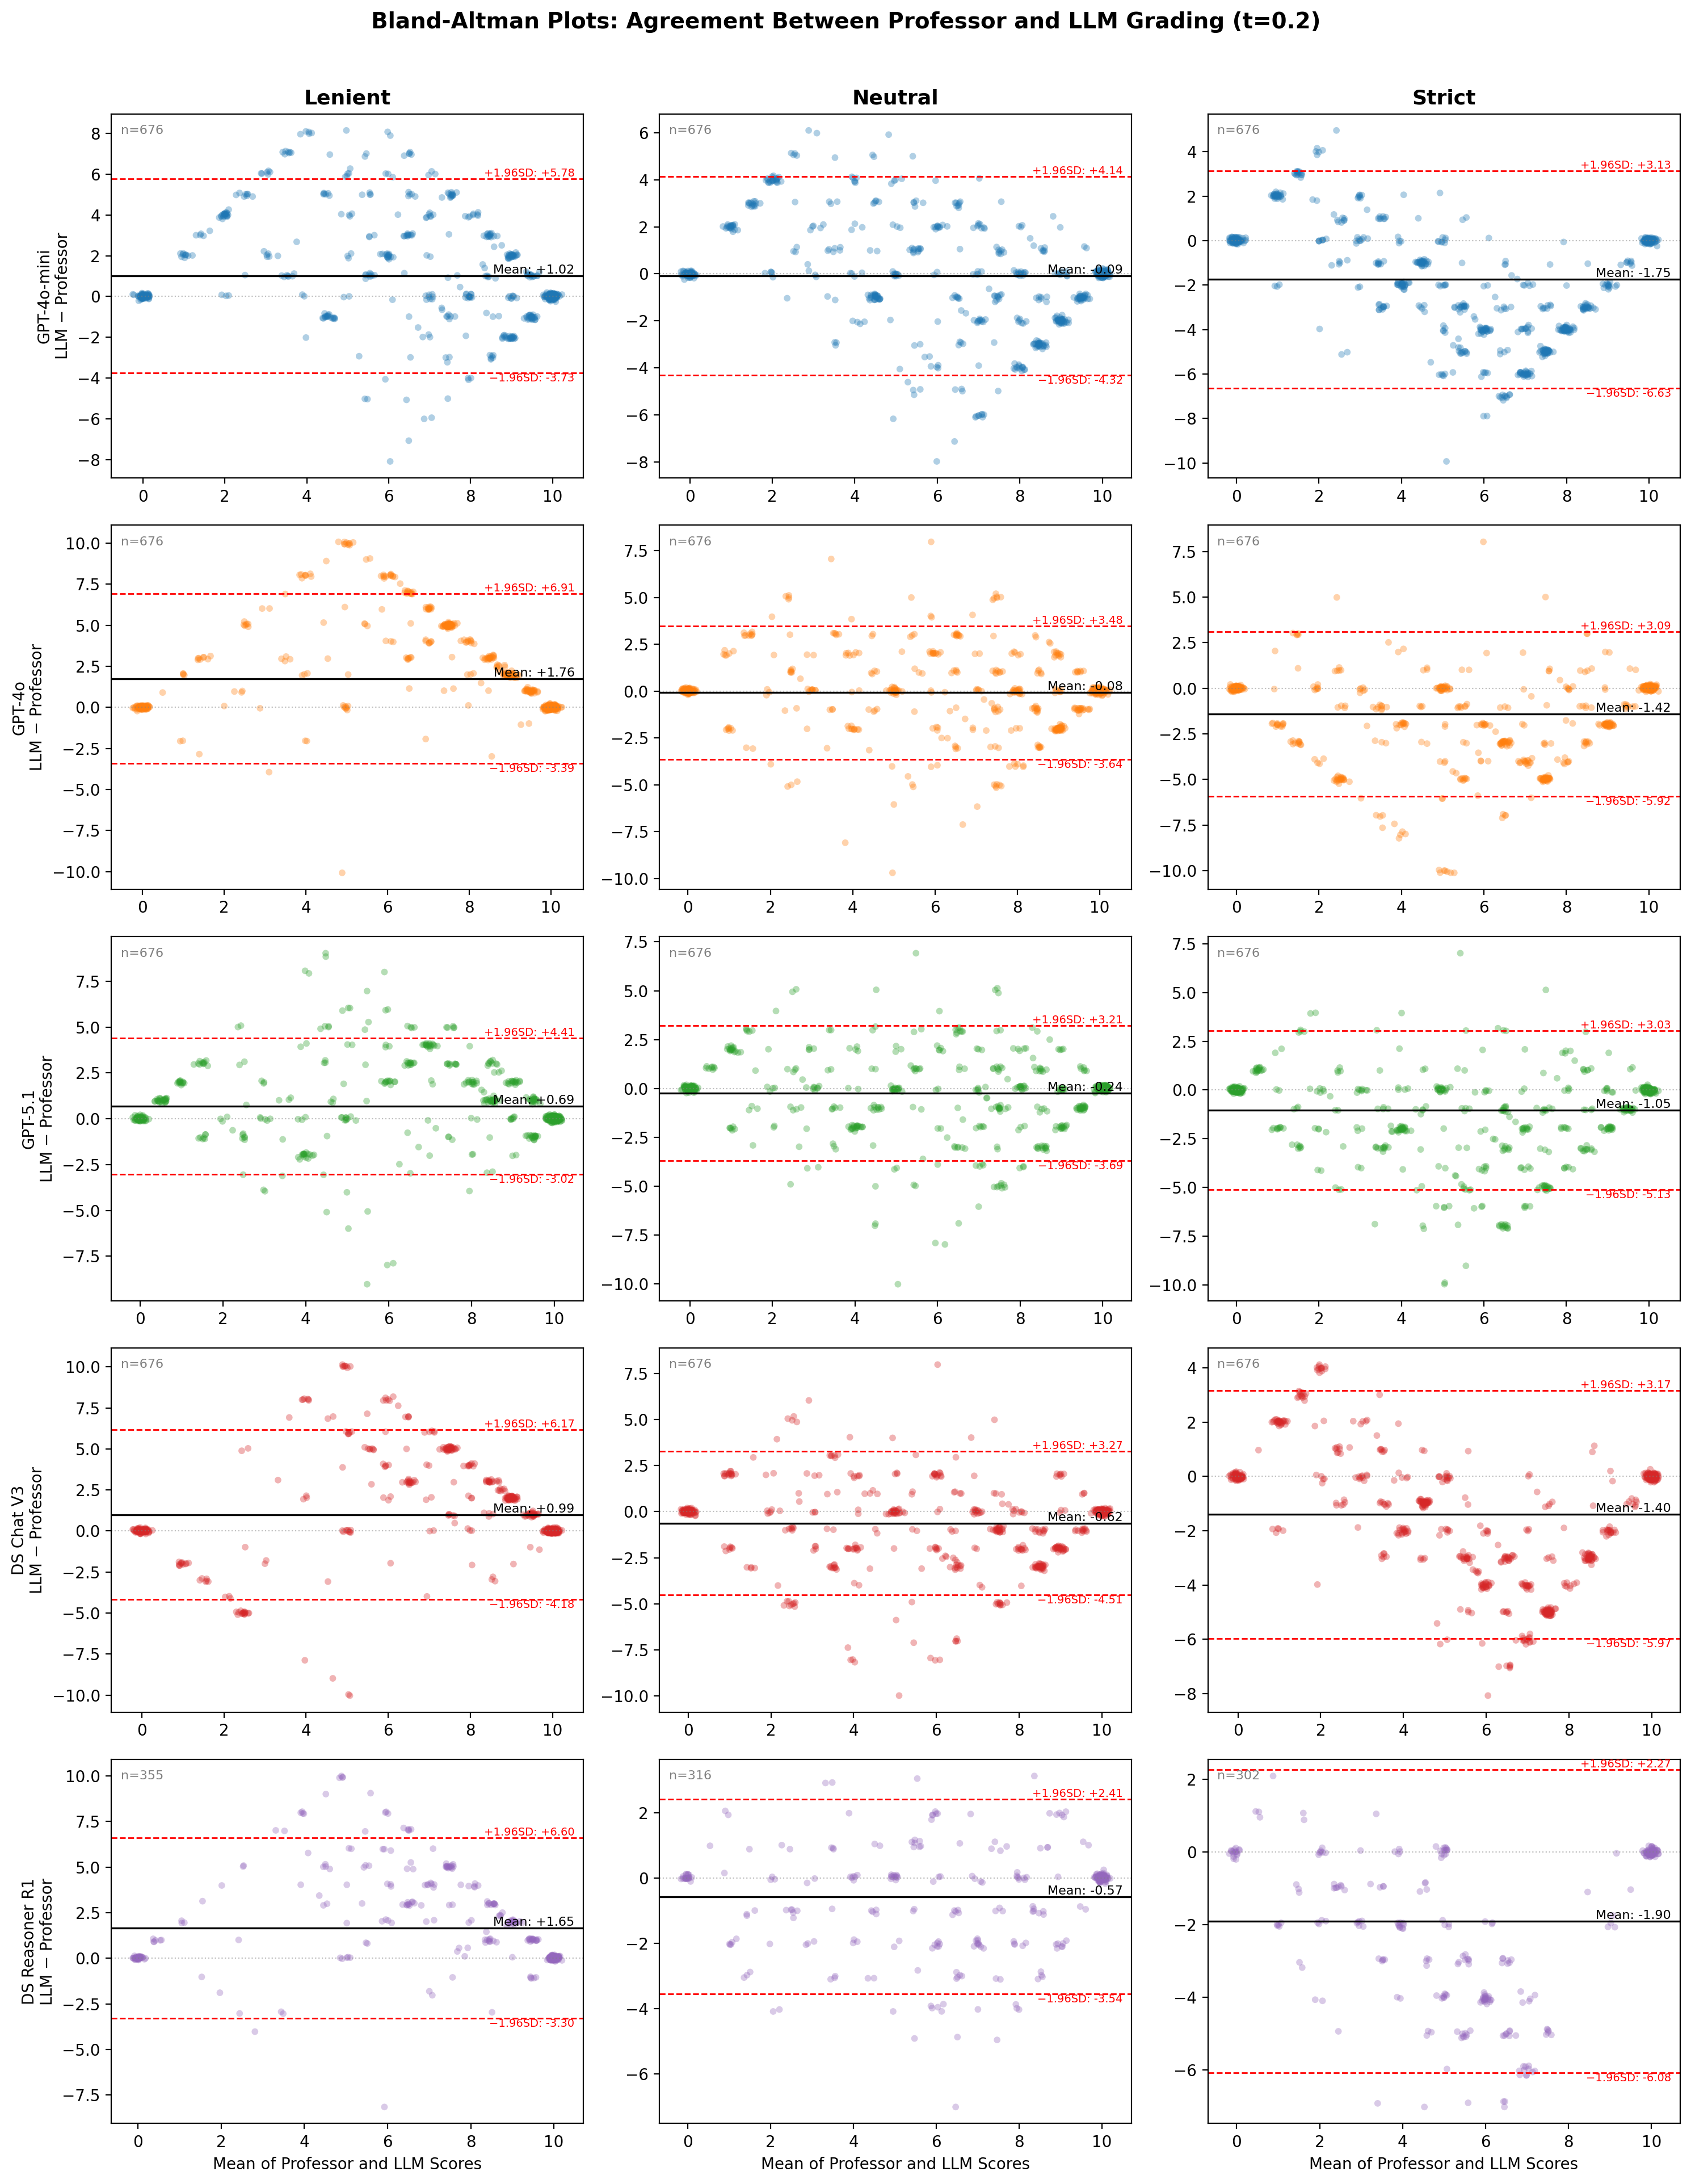
\includegraphics[width=\textwidth]{figures/bland_altman_pra.png}
\caption{Bland--Altmanovi dijagrami za PRA režim kroz sve modele i konfiguracije strogosti ($t=0{,}2$).
Svaka tačka predstavlja jedan ocenjeni studentski odgovor.}
\label{fig:ba_pra}
\end{figure}

\begin{figure}[ht!]
\centering
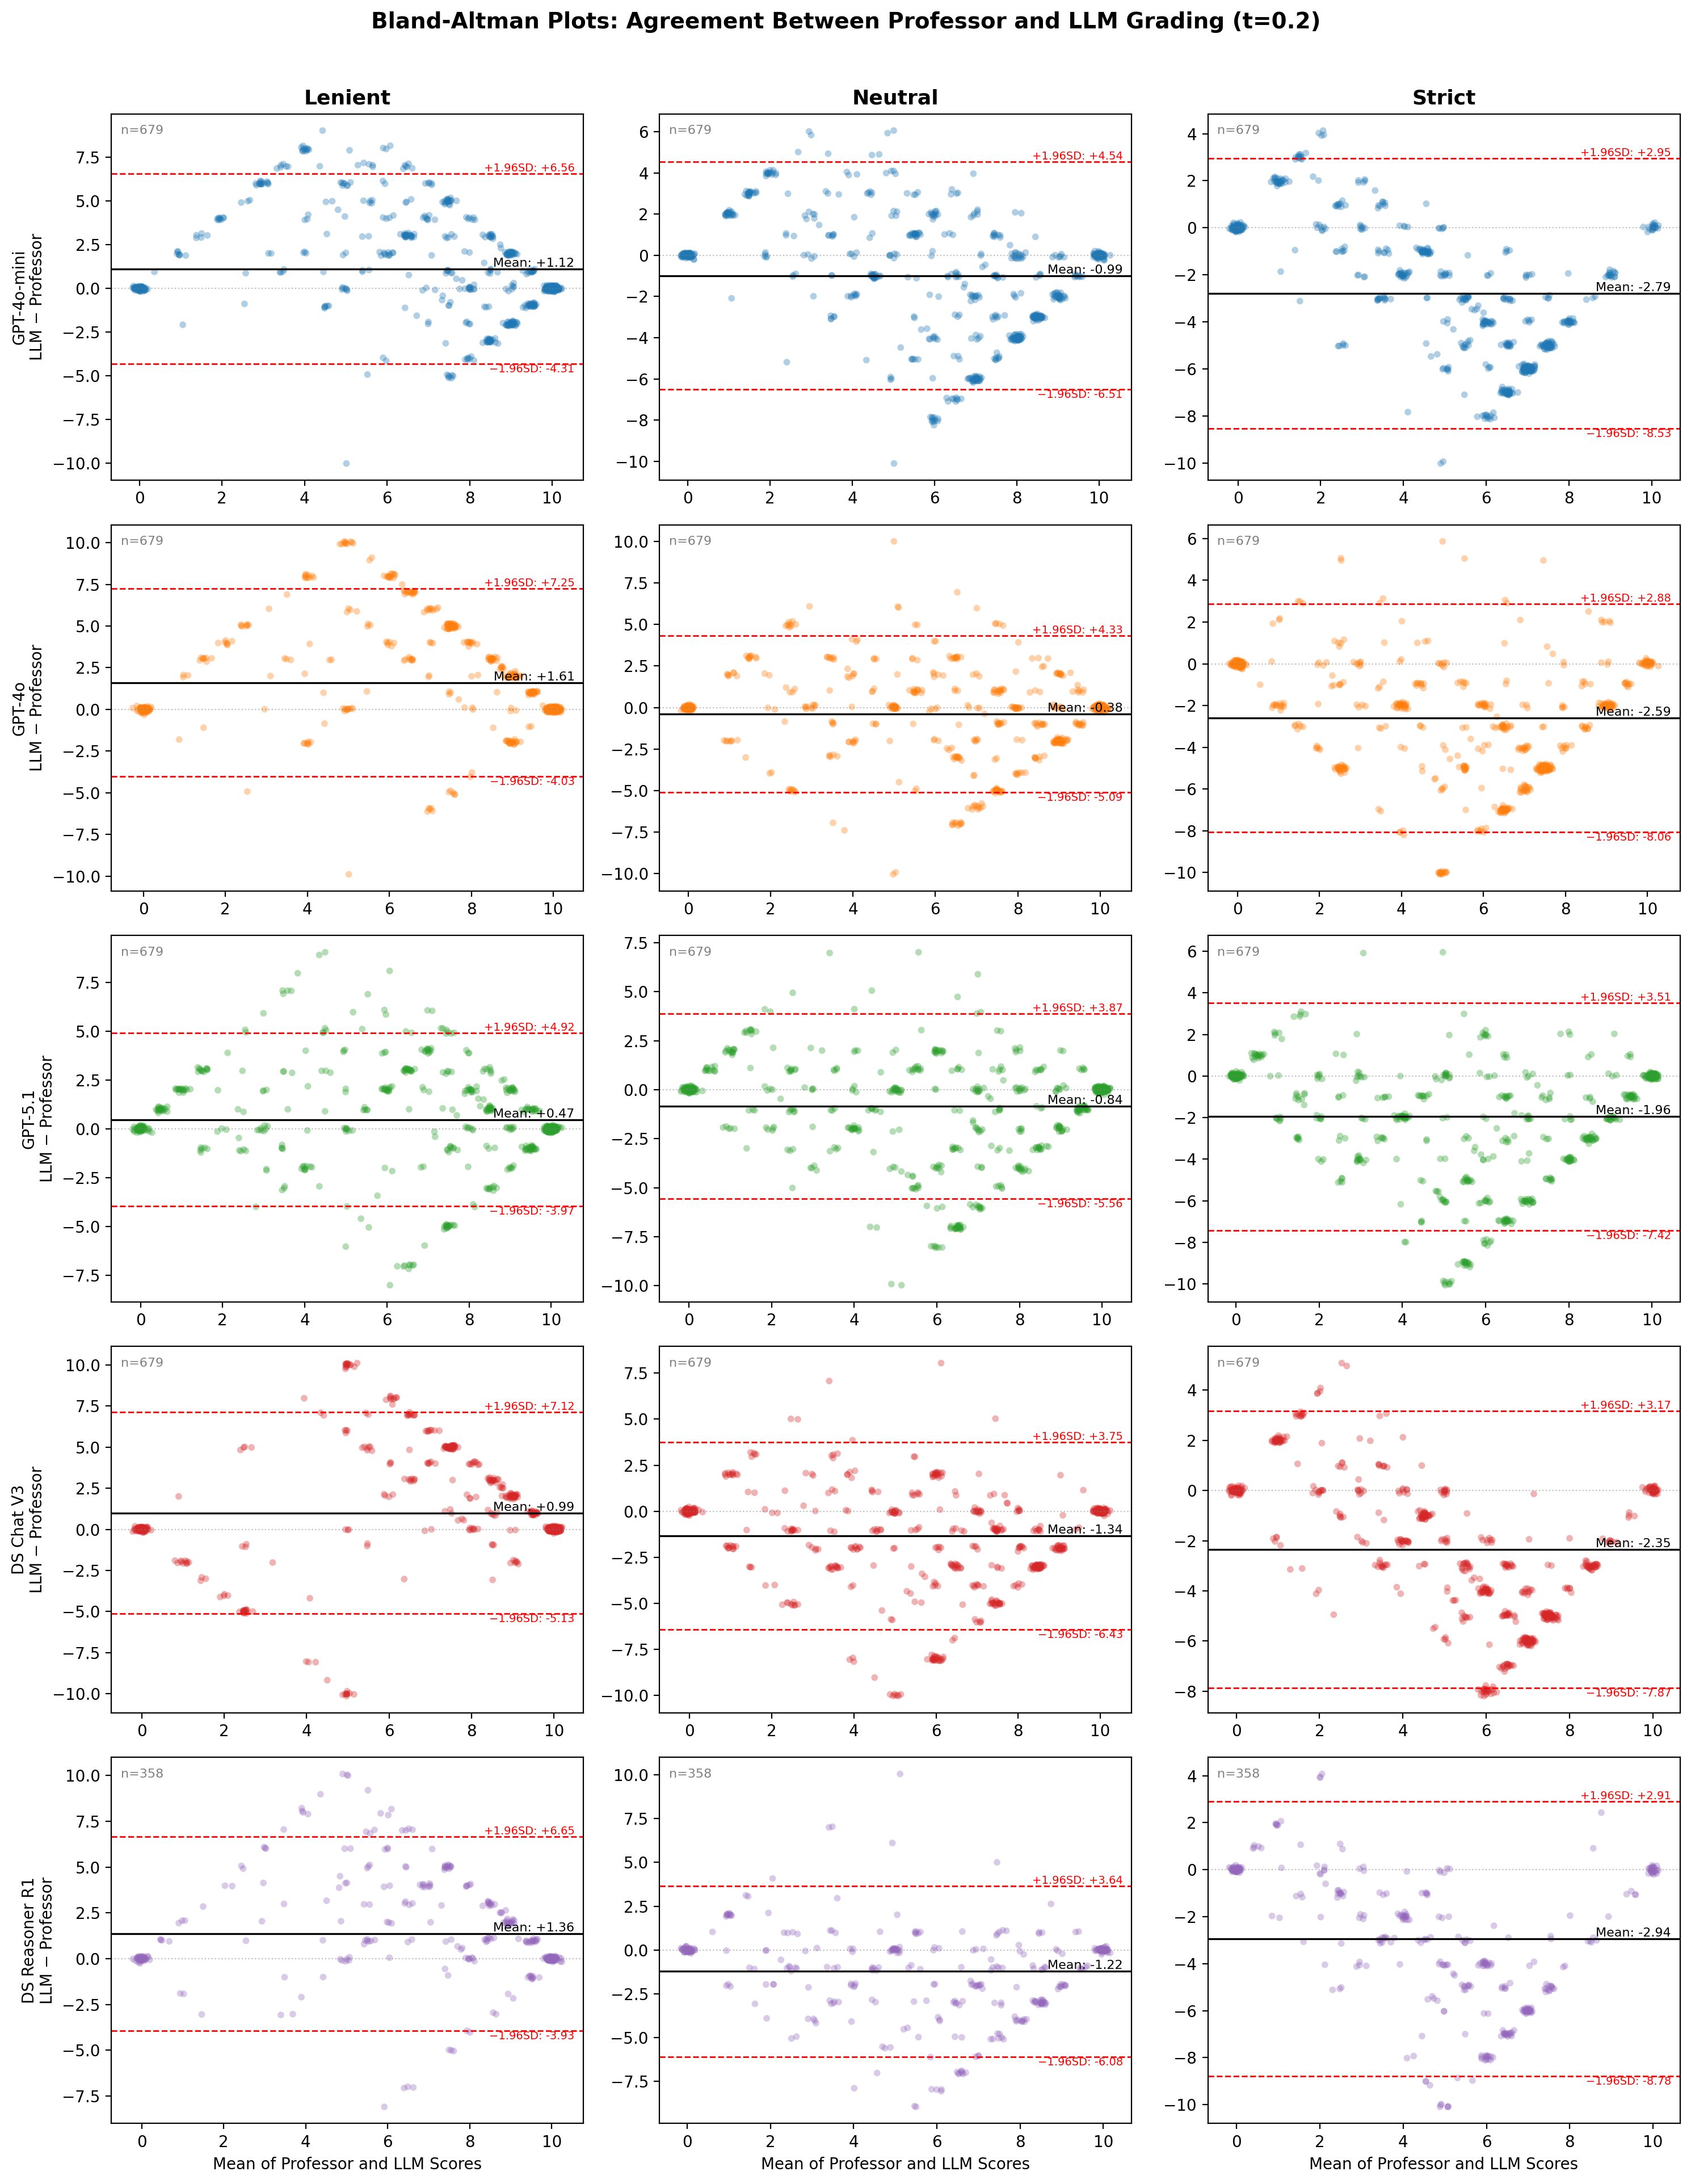
\includegraphics[width=\textwidth]{figures/bland_altman_gra.png}
\caption{Bland--Altmanovi dijagrami za GRA režim kroz sve modele i konfiguracije strogosti ($t=0{,}2$).}
\label{fig:ba_gra}
\end{figure}

\subsection{Analiza PCC-a po skupovima podataka}
\label{sec:cross-dataset}

Tabele~\ref{tab:pcc-reference-best} i~\ref{tab:pcc-generated-best} prikazuju vrednosti PCC-a kroz sve skupove podataka za PRA odnosno GRA ocenjivanje, koristeći neutralnu konfiguraciju za svaki model.
To omogućava poređenje modela u njihovim optimalnim konfiguracijama, umesto u jednoj fiksnoj globalnoj postavci.

Primetna razlika između PRA i GRA rezultata javlja se na kursevima gde se očekuje veoma kratak i precizan studentski odgovor, kao što su WP i TSW.
Na ovim skupovima podataka vrednosti PCC-a za GRA znatno opadaju u odnosu na PRA (tabela~\ref{tab:pcc-reference-best} naspram tabele~\ref{tab:pcc-generated-best}).
Jedan od razloga je taj što automatski generisani referentni odgovori teže da budu znatno duži i opisniji od sažetih rešenja koja daje nastavnik.
Kao posledica, model često dodeljuje visoke ocene odgovorima koji ispravno opisuju traženi postupak, ali ga zapravo ne izvršavaju.
Nasuprot tome, nastavnik je takve odgovore ocenjivao strogo i po pravilu dodeljivao nula poena kada tražena radnja nije sprovedena.
Ovaj raskorak između opisne i proceduralne tačnosti smanjuje slaganje sa ljudskim ocenjivanjem.

Ovakvo ponašanje može se ublažiti uključivanjem kratke napomene nastavnika koja eksplicitno naglašava da li je tačno objašnjenje samo po sebi dovoljno ili student mora u potpunosti da izvrši traženi zadatak.
Takvo usmerenje pomaže modelu da kriterijume ocenjivanja bolje uskladi sa očekivanjima nastavnika.

Kod skupova podataka gde se očekuju duži, opisniji odgovori (npr.\ DDS, DM i HTML5), razlike između PRA i GRA su znatno manje.
U tim slučajevima generisani referentni odgovori po strukturi i nivou detalja liče na odgovore nastavnika, što vodi sličnom ponašanju pri ocenjivanju i uporedivim vrednostima PCC-a u oba režima.

\begin{table}[ht]
\centering
\caption{PCC kroz sve skupove podataka za PRA režim (neutralna konfiguracija, temperatura 0{,}2; DeepSeek-Reasoner ne podržava podešavanje temperature)}
\label{tab:pcc-reference-best}
\resizebox{\columnwidth}{!}{%
\begin{tabular}{lccccc}
\toprule
\textbf{Skup podataka} & \textbf{DeepSeek-Chat} & \textbf{DeepSeek-Reasoner} & \textbf{GPT-4o} & \textbf{GPT-4o-mini} & \textbf{GPT-5.1} \\
\midrule
Prog 2 & 0.86 & 0.88 & \textbf{0.89} & 0.84 & \textbf{0.89} \\
TSW    & \textbf{0.94} & 0.88 & 0.92 & 0.91 & \textbf{0.94} \\
WP     & 0.78 & 0.67 & 0.78 & 0.77 & \textbf{0.87} \\
DDS    & 0.91 & 0.88 & 0.77 & \textbf{0.95} & 0.92 \\
HTML5  & 0.96 & 0.93 & \textbf{0.97} & 0.96 & \textbf{0.97} \\
DM     & 0.82 & 0.84 & 0.87 & 0.75 & \textbf{0.91} \\
\bottomrule
\end{tabular}
}
\end{table}

\begin{table}[ht]
\centering
\caption{Najbolji PCC kroz sve skupove podataka za GRA režim (temperatura 0{,}2; DeepSeek-Reasoner koristi temperaturu 0 jer ne podržava podešavanje temperature)}
\label{tab:pcc-generated-best}
\resizebox{\columnwidth}{!}{%
\begin{tabular}{lccccc}
\toprule
\textbf{Skup podataka} & \textbf{DeepSeek-Chat} & \textbf{DeepSeek-Reasoner} & \textbf{GPT-4o} & \textbf{GPT-4o-mini} & \textbf{GPT-5.1} \\
\midrule
Prog 2 & 0.78 & 0.81 & 0.80 & 0.76 & \textbf{0.84} \\
TSW    & 0.51 & 0.78 & \textbf{0.84} & 0.64 & 0.57 \\
WP     & 0.62 & 0.66 & \textbf{0.82} & 0.80 & 0.76 \\
DDS    & 0.81 & 0.66 & \textbf{0.89} & 0.87 & \textbf{0.89} \\
HTML5  & 0.95 & 0.92 & 0.98 & 0.97 & \textbf{0.99} \\
DM     & 0.82 & 0.83 & 0.85 & 0.75 & \textbf{0.92} \\
\bottomrule
\end{tabular}
}
\end{table}

\subsection{Stabilnost ocenjivanja kroz višestruka pokretanja}
\label{sec:stabilnost}

Budući da su izlazi velikih jezičkih modela inherentno stohastički, stabilnost ocenjivanja dodatno je procenjena ponavljanjem istog zadatka ocenjivanja tri nezavisna puta, koristeći GPT-5.1 sa temperaturom 0{,}2 i podrazumevanim (neutralnim) promptom strogosti.
Tabela~\ref{tab:variability} sumira rezultate.

Nad svih 686 pitanja, agregirane metrike pokazale su zanemarljivu varijaciju između pokretanja: PCC $= 0{,}899 \pm 0{,}002$, ponderisana kapa $= 0{,}896 \pm 0{,}002$, odnos prosečnih ocena $= 0{,}962 \pm 0{,}002$ i RMSE/STDDEV $= 0{,}448 \pm 0{,}003$.
Na nivou pojedinačnih pitanja, 82\% ocena bilo je identično u sva tri pokretanja, a 97\% se razlikovalo za najviše 1 poen na skali 0--10, uz prosečnu maksimalnu razliku od 0{,}21 poena.

Na nivou skupova podataka, varijabilnost je ostala niska u svim slučajevima, sa najmanjim standardnim devijacijama kod najstabilnijih podskupova i nešto višom varijabilnošću kod manjih skupova podataka.

\begin{table}[ht]
\centering
\caption{Analiza varijabilnosti ocenjivanja modela GPT-5.1 za PRA režim kroz tri nezavisna pokretanja ($t=0{,}2$, podrazumevana strogost).
Svako polje prikazuje prosek $\pm$ standardnu devijaciju nad 3 pokretanja.}
\label{tab:variability}
\resizebox{\columnwidth}{!}{%
\begin{tabular}{lcccc}
\toprule
\textbf{Skup podataka} & \textbf{PCC} & \textbf{Ponderisana kapa} & \textbf{Odnos proseka} & \textbf{RMSE/STDDEV} \\
\midrule
Prog 2 & 0.892 $\pm$ 0.002 & 0.888 $\pm$ 0.002 & 0.941 $\pm$ 0.002 & 0.464 $\pm$ 0.004 \\
TSW    & 0.953 $\pm$ 0.006 & 0.886 $\pm$ 0.013 & 0.979 $\pm$ 0.002 & 0.328 $\pm$ 0.026 \\
WP     & 0.855 $\pm$ 0.006 & 0.747 $\pm$ 0.011 & 0.930 $\pm$ 0.002 & 0.694 $\pm$ 0.030 \\
DDS    & 0.882 $\pm$ 0.016 & 0.823 $\pm$ 0.034 & 0.869 $\pm$ 0.010 & 0.622 $\pm$ 0.026 \\
HTML5  & 0.969 $\pm$ 0.004 & 0.959 $\pm$ 0.006 & 0.898 $\pm$ 0.008 & 0.311 $\pm$ 0.019 \\
DM     & 0.915 $\pm$ 0.005 & 0.894 $\pm$ 0.005 & 1.109 $\pm$ 0.003 & 0.466 $\pm$ 0.012 \\
\midrule
SVI    & 0.899 $\pm$ 0.002 & 0.896 $\pm$ 0.002 & 0.962 $\pm$ 0.002 & 0.448 $\pm$ 0.003 \\
\bottomrule
\end{tabular}
}
\end{table}

% 6. Diskusija
\section{Diskusija}
\label{sec:diskusija}

\subsection{Poređenje sa prethodnim istraživanjima}
\label{sec:poredjenje}

Da bi se dobijeni rezultati smestili u kontekst šire literature, tabela~\ref{tab:prior-study} poredi vrednosti PCC-a postignute u ovom istraživanju sa vrednostima iz prethodnih studija.
Kao što se vidi, EduGrader --- naročito sa modelom za rezonovanje GPT-5.1 --- postiže znatno višu usklađenost između veštačke inteligencije i ljudskih ocenjivača od objavljenih rezultata sa kojima je poređen.

\begin{table}[ht]
\centering
\caption{Poređenje sa prethodno objavljenim rezultatima}
\label{tab:prior-study}
\begin{tabular}{lll}
\toprule
Pristup & Model & PCC \\
\midrule
Jukjevič~\cite{jukiewicz2024future}       & gpt-3.5-turbo & 0.81 \\
Kuli i Jusuf~\cite{kooli2025transforming} & ChatGPT       & 0.45 \\
Lundgren~\cite{lundgren2024large}         & gpt-4         & 0.43 \\
Naš pristup                               & gpt-5.1       & \textbf{0.90} \\
\bottomrule
\end{tabular}
\end{table}

U našim eksperimentima, najbolja konfiguracija (GPT-5.1, neutralna strogost) postiže PCC $= 0{,}90$, čime premašuje vrednost koju je prijavio Jukjevič (0{,}81, koristeći gpt-3.5-turbo za ocenjivanje programerskih zadataka)~\cite{jukiewicz2024future} i znatno nadmašuje korelacije iz studija koje su koristile ChatGPT ili GPT-4 za ocenjivanje odgovora otvorenog tipa i eseja (PCC $= 0{,}43$--$0{,}45$)~\cite{kooli2025transforming,lundgren2024large}.
Iako ova poređenja treba tumačiti sa oprezom zbog razlika u skupovima podataka i formatima zadataka, dva faktora verovatno doprinose višoj usklađenosti u našoj postavci.
Prvo, EduGrader evaluira širi skup savremenih modela, uključujući GPT-4o, GPT-4o-mini, DeepSeek-Chat i, posebno, modele usmerene na rezonovanje (GPT-5.1, DeepSeek-Reasoner).
Ovi modeli pokazuju snažnije semantičko razumevanje i stabilnije ponašanje kroz konfiguracije strogosti, što se ogleda ne samo u višim vrednostima PCC-a već i u nižim odnosima RMSE/STDDEV, koji se često približavaju tipičnoj varijabilnosti ljudskog ocenjivanja.
Drugo, zadaci u našem skupu podataka sastoje se prvenstveno od kratkih teorijskih pitanja iz STEM oblasti (nauka, tehnologija, inženjerstvo i matematika).
Očekivani odgovori su često kratka tekstualna objašnjenja ili mali izrazi nalik kodu, koji su po pravilu manje dvosmisleni od dugih eseja u društvenim ili političkim naukama.
Vredi napomenuti i da su naši nalazi u skladu sa prethodnim istraživanjima po tome što su ljudski ocenjivači u proseku nešto blaži, pokazujući veću toleranciju prema delimično ispravnom rezonovanju i nepotpunim odgovorima~\cite{jukiewicz2024future}.

\subsection{Ograničenja}
\label{sec:ogranicenja}

Uprkos snažnim ukupnim performansama, ograničenja ostaju: ponašanje modela može se promeniti kako se API-ji razvijaju, evaluacioni skup podataka je vezan za konkretne domene, a povremeno prestrogo kažnjavanje ili pogrešno tumačenje odgovora i dalje je moguće.
Iz ovih razloga, ljudski nadzor ostaje neophodan.
EduGrader je zamišljen kao pomoćni sistem koji unapređuje doslednost i smanjuje opterećenje nastavnika, uz očuvanje autoriteta nastavnika za dvosmislene slučajeve i konačne odluke o ocenama.
U toj ulozi, podesiva strogost i objašnjiva povratna informacija čine EduGrader praktičnom i transparentnom dopunom tradicionalnih tokova provere znanja.

\subsection{Pravci budućeg rada}
\label{sec:buduci-rad}

Nekoliko pravaca može dodatno unaprediti tačnost, robusnost i pedagoški uticaj sistema EduGrader:
\begin{itemize}
    \item \textbf{Samoprovera i probni ispiti:} omogućiti studentima da iz nastavnih materijala generišu personalizovana probna pitanja i dobijaju kontinuiranu formativnu povratnu informaciju tokom semestra.
    \item \textbf{Usmeravanje zasnovano na pouzdanosti:} analizirati slaganje između više jezičkih modela radi procene pouzdanosti ocene.
    Slučajevi niske pouzdanosti mogu se automatski označavati za pojačanu pažnju nastavnika, čime se obezbeđuje pouzdaniji nadzor.
    \item \textbf{Ansambl ocenjivanje:} kombinovati modele za rezonovanje i standardne modele (npr.\ usrednjavanjem ili većinskim glasanjem) radi stabilnijih i robusnijih ishoda ocenjivanja nego što ih daje bilo koji pojedinačni model.
    \item \textbf{Longitudinalna kalibracija:} pratiti raskorake između ocena sistema i nastavnika kroz više semestara, radi automatskog podešavanja parametara strogosti i održavanja doslednih standarda ocenjivanja tokom vremena.
    \item \textbf{Proširenje domena i jezika:} evaluirati EduGrader na dugim esejskim zadacima, kreativnim zadacima i višejezičnim okruženjima, kako bi se ispitala njegova uopštivost izvan STEM disciplina, koje po pravilu uključuju strukturiranije i manje dvosmislene odgovore.
\end{itemize}

% 7. Zaključak
\section{Zaključak}
\label{sec:zakljucak}

U ovom radu predstavljen je EduGrader, višemodelska platforma otvorenog koda za ocenjivanje pitanja otvorenog tipa uz podršku veštačke inteligencije i pod nadzorom nastavnika.
Sistem objedinjuje više velikih jezičkih modela (GPT-4o, GPT-4o-mini, DeepSeek-Chat i dva modela usmerena na rezonovanje, GPT-5.1 i DeepSeek-Reasoner) u podesiv tok ocenjivanja koji podržava evaluaciju i u PRA i u GRA režimu.
EduGrader je evaluiran na 686 autentičnih studentskih odgovora sa šest univerzitetskih kurseva na dve institucije, koji obuhvataju kratke činjeničke odgovore, teorijska objašnjenja, izraze nalik kodu i dodatni skup dužih odgovora esejskog tipa.

Empirijski rezultati pokazuju da PRA režim dosledno daje višu usklađenost sa ljudskim ocenjivačima od GRA režima, kroz sve modele i konfiguracije strogosti.
Modeli usmereni na rezonovanje, naročito GPT-5.1, postižu najjače slaganje sa ljudskim ocenjivanjem, dostižući Pirsonov koeficijent korelacije od 0{,}90 u neutralnom PRA režimu.
Ovi ishodi povoljno se porede sa prethodno objavljenim rezultatima u literaturi i sugerišu da, za evaluirane tipove odgovora --- a posebno za relativno strukturirana STEM pitanja --- savremeni veliki jezički modeli mogu aproksimirati obrasce ljudskog ocenjivanja sa odstupanjima uporedivim sa prirodnom ljudskom varijabilnošću.
Istovremeno, analize otkrivaju sistematske razlike između modela, režima ocenjivanja i konfiguracija strogosti, što naglašava važnost pažljivog izbora modela i parametara pri stvarnoj primeni.

Iako EduGrader donosi značajne dobitke u efikasnosti, podesivu strogost i detaljno generisanje povratnih informacija, rezultati potvrđuju da su sistemi veštačke inteligencije najefikasniji kada se koriste kao pomoćni alati, a ne kao zamena za čoveka.
Ljudski nadzor ostaje neophodan za pravednost, kontekstualno tumačenje i rešavanje dvosmislenih ili graničnih slučajeva.

Objavljivanjem sistema EduGrader kao projekta otvorenog koda nastoji se podstaći transparentnost, reproducibilnost i zajedničko unapređivanje sistema.


% ------------------------------------------------------------
% Literatura
% ------------------------------------------------------------
\bibliographystyle{plain}
\bibliography{literatura}

% ------------------------------------------------------------
% Dodaci
% ------------------------------------------------------------
\appendix
% Dodatak A: Šabloni promptova i primeri ocenjivanja
\section{Šabloni promptova i primeri ocenjivanja}
\label{app:promptovi}

Ovaj dodatak sadrži materijale koji podržavaju transparentnost i reproducibilnost sistema EduGrader: osnovne šablone promptova korišćene u eksperimentima i nekoliko reprezentativnih primera ocenjivanja koje je sistem proizveo.
Šabloni promptova opisuju kako se studentski odgovori evaluiraju pod različitim konfiguracijama strogosti.
Prikazani su originalni promptovi korišćeni u eksperimentima.

\medskip
\noindent\textbf{Napomena.} Ocene su prikazane na skali 0--10.

\subsection*{Prompt za blago ocenjivanje}

\begin{tcolorbox}[promptbox]

Ti si veoma blag profesor koji ocenjuje studentske odgovore.

\vspace{2mm}

\textbf{Pravila ocenjivanja:}

\begin{itemize}[leftmargin=1.5em]
\item Cilj je da se prepozna razumevanje koncepta bez obzira na formulaciju odgovora.
\item Nedostajući detalji ili neprecizna terminologija se ne kažnjavaju.
\item Sinonimi, parafraziranje i primeri su prihvatljivi.
\item Kazni samo odgovore koji pokazuju potpuno pogrešno razumevanje ili su van teme.
\item U slučaju nedoumice dodeli više poena.
\item Prazan odgovor dobija 0 poena.
\end{itemize}

\end{tcolorbox}

\subsection*{Podrazumevani prompt (neutralna konfiguracija)}

\begin{tcolorbox}[promptbox]

Ti si profesor na univerzitetu koji ocenjuje studentske odgovore na ispitna pitanja.

\vspace{2mm}

\textbf{Pravila ocenjivanja:}

\begin{itemize}[leftmargin=1.5em]
\item Uporedi studentski odgovor sa tačnim odgovorom i proceni stepen poklapanja.
\item Odgovor ne mora biti identičan tačnom odgovoru ako student pokazuje razumevanje koncepta.
\item Sinonimi, parafraziranje i drugačiji redosled informacija su prihvatljivi ako je suština tačna.
\item Odgovori napisani na različitim jezicima ili pismima (ćirilica/latinica, srpski/engleski) ne treba da budu kažnjeni ako je sadržaj tačan.
\item Ako je odgovor delimično tačan, dodeli proporcionalan broj poena.
\item Ako odgovor sadrži netačne tvrdnje koje nisu deo tačnog odgovora, oduzmi poene proporcionalno.
\end{itemize}

\end{tcolorbox}

\subsection*{Prompt za strogo ocenjivanje}

\begin{tcolorbox}[promptbox]

Ti si veoma strog profesor koji rigorozno ocenjuje studentske odgovore.

\vspace{2mm}

\textbf{Pravila ocenjivanja:}

\begin{itemize}[leftmargin=1.5em]
\item Strogo uporedi studentski odgovor sa tačnim odgovorom.
\item Svaka stavka iz tačnog odgovora koja nedostaje znači oduzimanje poena.
\item Netačne ili neprecizne tvrdnje se kažnjavaju.
\item Površni ili previše opšti odgovori bez konkretnih detalja dobijaju manje poena.
\item Nepotpun odgovor ne može dobiti više od polovine poena.
\item Sinonimi i parafraziranje su prihvatljivi samo ako precizno pokrivaju suštinu tačnog odgovora.
\end{itemize}

\end{tcolorbox}

\subsection*{Reprezentativni primeri ocenjivanja}

Naredni primeri ilustruju tipične izlaze sistema EduGrader.

\subsection*{Primer A: Detekcija stepena broja dva}

\begin{tcolorbox}[promptbox]

\textbf{Pitanje}

Napisati C funkciju koja vraća 1 ako je broj stepen broja dva, a 0 u suprotnom.

\medskip
\textbf{Referentni odgovor}

\begin{verbatim}
int isPowerOfTwo(unsigned x) {
    return x != 0 && (x & (x - 1)) == 0;
}
\end{verbatim}

\medskip
\textbf{Studentski odgovor}

\begin{verbatim}
int isPowerOfTwo(unsigned x) {
    return (x & (x - 1)) == 0;
}
\end{verbatim}

\medskip
\textbf{Ocene}

Nastavnik: 7/10 \hfill Sistem: 8/10

\medskip
\textbf{Obrazloženje sistema}

Student pravilno primenjuje standardnu bitovsku tehniku za detekciju stepena broja dva koristeći izraz \texttt{(x \& (x - 1)) == 0}.
Međutim, rešenje ne obrađuje granični slučaj kada je \texttt{x == 0}.
Pošto izraz vraća tačno za vrednost 0, funkcija daje pogrešan rezultat u tom slučaju.
Rešenje je gotovo tačno, ali nije potpuno.

\end{tcolorbox}

\subsection*{Primer B: Stek i hip memorija}

\begin{tcolorbox}[promptbox]

\textbf{Pitanje}

Koja je razlika između stek memorije i hip memorije u C-u?
Ukratko objasniti.

\medskip
\textbf{Studentski odgovor}

Stek je memorija koju program koristi za pozive funkcija i lokalne promenljive.
Hip je memorija koja čuva globalne promenljive i velike podatke.
Stek je brži, hip je sporiji.

\medskip
\textbf{Ocene}

Nastavnik: 6/10 \hfill Sistem: 6/10

\medskip
\textbf{Obrazloženje sistema}

Student tačno navodi da se stek koristi za pozive funkcija i lokalne promenljive i da je generalno brži.
Međutim, tvrdnja da hip čuva globalne promenljive je netačna.
Globalne promenljive se nalaze u statičkoj memoriji, a ne u hipu.
Takođe, odgovor ne objašnjava dinamičku alokaciju niti razlike u životnom veku memorije.

\end{tcolorbox}


\end{document}
